\chapter{Simulating GOTO Observations}
\label{chap:sims}
\chaptoc{}

% ########################################

\newpage
\section{Introduction}
\label{sec:sims_intro}
\begin{colsection}

% ~~~~~~~~~~~~~~~~~~~~

\begin{colsection}

In this chapter I outline my work creating simulations of the GOTO observatory. Section~\ref{sec:scheduler_sims} describes early simulations carried out in order to find the optimal ``tie-break'' parameters for the \gls{gtecs} scheduler, Section~\ref{sec:multi_site} details how this simulation code could be modified to simulate multiple observing sites and Sections~\ref{sec:gw_sims} and~\ref{sec:survey_sims} apply this to multi-site simulations of gravitational wave events and the all-sky survey respectively. All work described in this chapter is my own and has not been published before anywhere else.

\end{colsection}

% ~~~~~~~~~~~~~~~~~~~~

\subsection{Simulating GOTO}
\label{sec:goto_sims}
\begin{colsection}

\rtxt{Describe the fake pilot here, it's common to all 3 sims}.

Below is taken from the old multi-site sim section, needs improvement.

As described in Section~\ref{sec:goto_expansion}, the ultimate aim of the \gls{goto} project is to have multiple nodes around the world. Specifically, the plan calls for two full GOTO-8 systems on La Palma and another two at a second site in Australia (the exact site is not yet determined, but it will most likely either be either Siding Spring in New South Wales or Mt Kent in Queensland).

In order to better quantify the benefit multiple telescopes and sites will provide, a series of simulations were carried out. These simulations focused on two main areas: the all-sky survey coverage and cadence, and the combined system's response to gravitational wave alerts.

\end{colsection}

% ~~~~~~~~~~~~~~~~~~~~

\end{colsection}

% ########################################

\newpage
\section{Scheduler simulations}
\label{sec:scheduler_sims}
\begin{colsection}

% ~~~~~~~~~~~~~~~~~~~~

\begin{colsection}

The first simulations of the \gls{gtecs} system were carried out in 2016 when the target scheduling code was being written. The scheduler needs a way to distinguish equally-ranked pointings, as described below, and the choice of weightings for this `tiebreaker' needed to be decided on. Therefore a series of simulations were carried out in order to find which weightings gave the best performance when observing gravitational wave skymaps.

\end{colsection}

% ~~~~~~~~~~~~~~~~~~~~

\subsection{The scheduler tiebreaker}
\label{sec:scheduler_tiebreaker}
\begin{colsection}

The workings of the scheduler functions are described in detail in Section~\ref{sec:scheduler}. The scheduler weights pointings in the current queue by several parameters: the assigned rank, the number of times it was previously observed, if it is a \gls{too} or not. But in practice most of the time the queue will contain a large number of pointings where these values are all the same. For example, when a new gravitational wave event is processed by the sentinel GOTO-alert adds in a large number of tiles from the skymap (see \aref{sec:db_insert}). On the next scheduler check the queue will be populated by a large number of pointings each with the same rank and \gls{too} flag and having never been observed. Likewise when observing the all-sky survey the queue will be filled with tiles that have all been observed the same number of times. This is why the scheduler then needs a further way to distinguish pointings, which is known as the tiebreaker.

The pre-existing \gls{pt5m} scheduling code (see \aref{sec:pt5m}) used only a single parameter to decide between equally-ranked pointings: the airmass each target would be at at the midpoint of the observation (The scheduler constraints are applied at both the start and stop times of the observation, to ensure that the target remains visible throughout (unlike GOTO, which only observes targets for a few minutes, \gls{pt5m} often observes the same target for several hours at a time). For the tiebreaker the airmass is calculated at the midpoint of this observation period.). This works well to prioritise getting the best data quality, assuming the two targets are otherwise identical.

% ---------
\subsubsection{Tile weighting}

When adapting the \gls{pt5m} system for GOTO it was clear there was the need for an additional parameter in the scheduling functions, to encode the relative weights of a set of pointings. All the pointings added from a gravitational wave skymap (or similar event such as a gamma-ray burst) will have the same rank, but they will have different weights from the amount of skymap probability they each contain. It makes sense that, of all the tiles from a given event, the ones with higher probability should be the ones to prioritise and observe first. However unlike an integer parameter such as the rank or the \gls{too} flag the tile weights cover a wide range and often there will only be a small amount of difference between the values for neighbouring tiles. Prioritising a tile that contains 2.71\% of the skymap over another that contains 2.70\% in all cases is not the best strategy, especially if the latter is close to zenith while the former is very low down. Observing a high-airmass tile over a low-airmass one for a gain of only 0.01\% probability is a poor choice, especially if the former tile is currently rising and will be at a better altitude in a few hours. For these reasons it was decided that the skymap probability weighting should be considered at the same level as the airmass tiebreaker, meaning a lower-airmass tile with only a slightly power probability will be prioritised over one further from zenith. This should only be true up to a reasonable limit however, in the case of two tiles where one contains 95\% and the other 3\% it should always be true that observing the latter is the better choice, even if it has a slightly worse airmass.

It should be noted that probability is not necessarily the only way for a group of tiles to be weighted. In the past GOTO has carried out more focused surveys: in the galaxy survey for example tiles were weighted by the total flux of all galaxies within each tile, which is not strictly a probability. As this section deals exclusively with gravitational wave skymaps the term `probability' rather than `weight' will be used to describe the relative measure of each tile to the others added from the same event, even though the latter is used in the \gls{gtecs} scheduler code. This also avoids confusion when later discussing the relative weighting between probability and airmass in the tiebreaker ratio.

% ---------
\subsubsection{Airmass vs time-to-set}

Airmass is usually modelled using a plane-parallel atmosphere as $X=\sec{z}$, where $X$ is airmass and $z$ is the zenith angle ($z=90-h$ where $h$ is the altitude of the target). This makes it by definition an entirely symmetric parameter around the zenith, with no consideration for is a target is rising or setting. This was identified as a problem for similar reasons given above. Consider the scenario where there are two tiles with equal or similar contained probabilities, but one is \SI{5}{\degree} above the horizon in the west and the other is \SI{10}{\degree} above the horizon in in the east. The one in the west will be setting while the one in the east wil lbe rising, and that naturally means that the system should prioritise the one in the west as unless it is observed quickly it will pass below the horizon and no longer be visible for the remainder of the night.

In order to correct this problem, it was required that the airmass value be replaced by a different parameter that will prioritise targets that are about to set. This new parameter is called `time-to-set', and is simply the time until the target sets below the defined horizon. The units are arbitrary, but as it will repeat with a period of 24 hours the time-to-set value is normalised between 0 and 1 so that 0 is when the target is at the horizon, 0.5 is when it is 12 hours from setting and 1 is 24 hours from setting (and there is therefore a degeneracy at 0 and 1). \aref{fig:airmass_tts} shows how altitude, airmass and time-to-set are defined for any non-circumpolar target. Circumpolar targets are ones that never set below the horizon, and therefore the time-to-set is an illogical value. However as from La Palma the North Pole is just below the \SI{30}{\degree} horizon limit this is not a concern for GOTO and is therefore not considered.

Purely replacing airmass with the time-to-set would not produce good results, as the telescope would be prioritised to constantly be observing the western horizon. As with probability, a weighted combination of the two would be best in order to take both parameters into account. However exactly how to combine the two is not a simple problem. \aref{fig:at_ratio} shows how combining airmass and time-to-set, both normalised to between 0 and 1, produces a new distribution. As the ratio the two are combined with is increased in favour of time-to-set the peak of the distribution shifts to favour targets that are setting over those at the zenith.

\begin{figure}[p]
    \begin{center}
        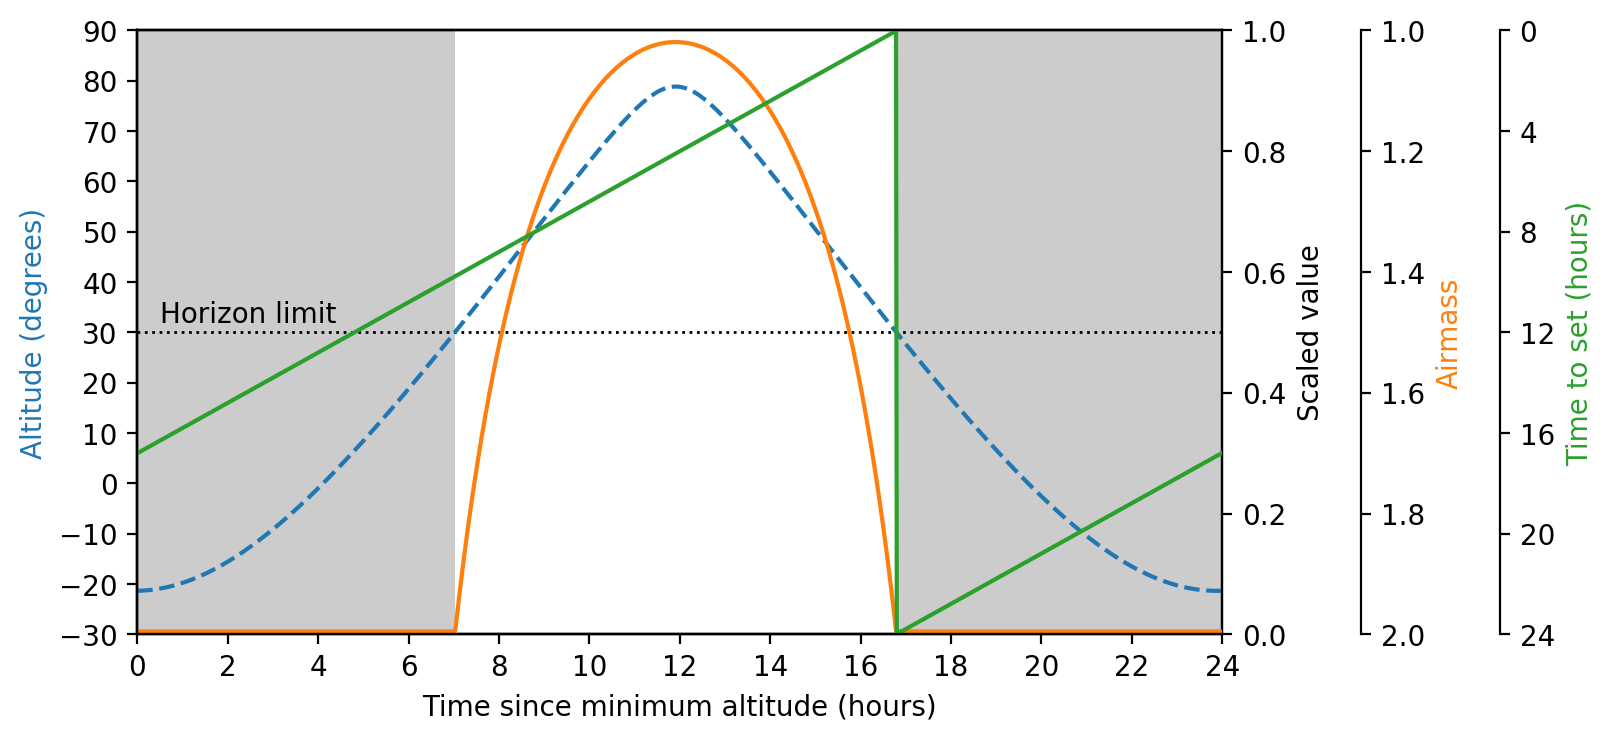
\includegraphics[width=\linewidth]{images/airmass-tts.png}
    \end{center}
    \caption[Defining airmass and time-to-set for a given target]{
        Defining airmass and time-to-set for a particular, arbitrary target. The altitude of the target is shown in \textcolor{Blue}{blue} over the course of one day and the corresponding airmass in \textcolor{BurntOrange}{orange}. The time-to-set is shown in \textcolor{Green}{green}, decreasing to 0 at the time the target passes below the \SI{30}{\degree} horizon (shown in red) and then resetting to the maximum. The grey regions are the times when the target is below the horizon.
    }\label{fig:airmass_tts}
\end{figure}

\begin{figure}[p]
    \begin{center}
        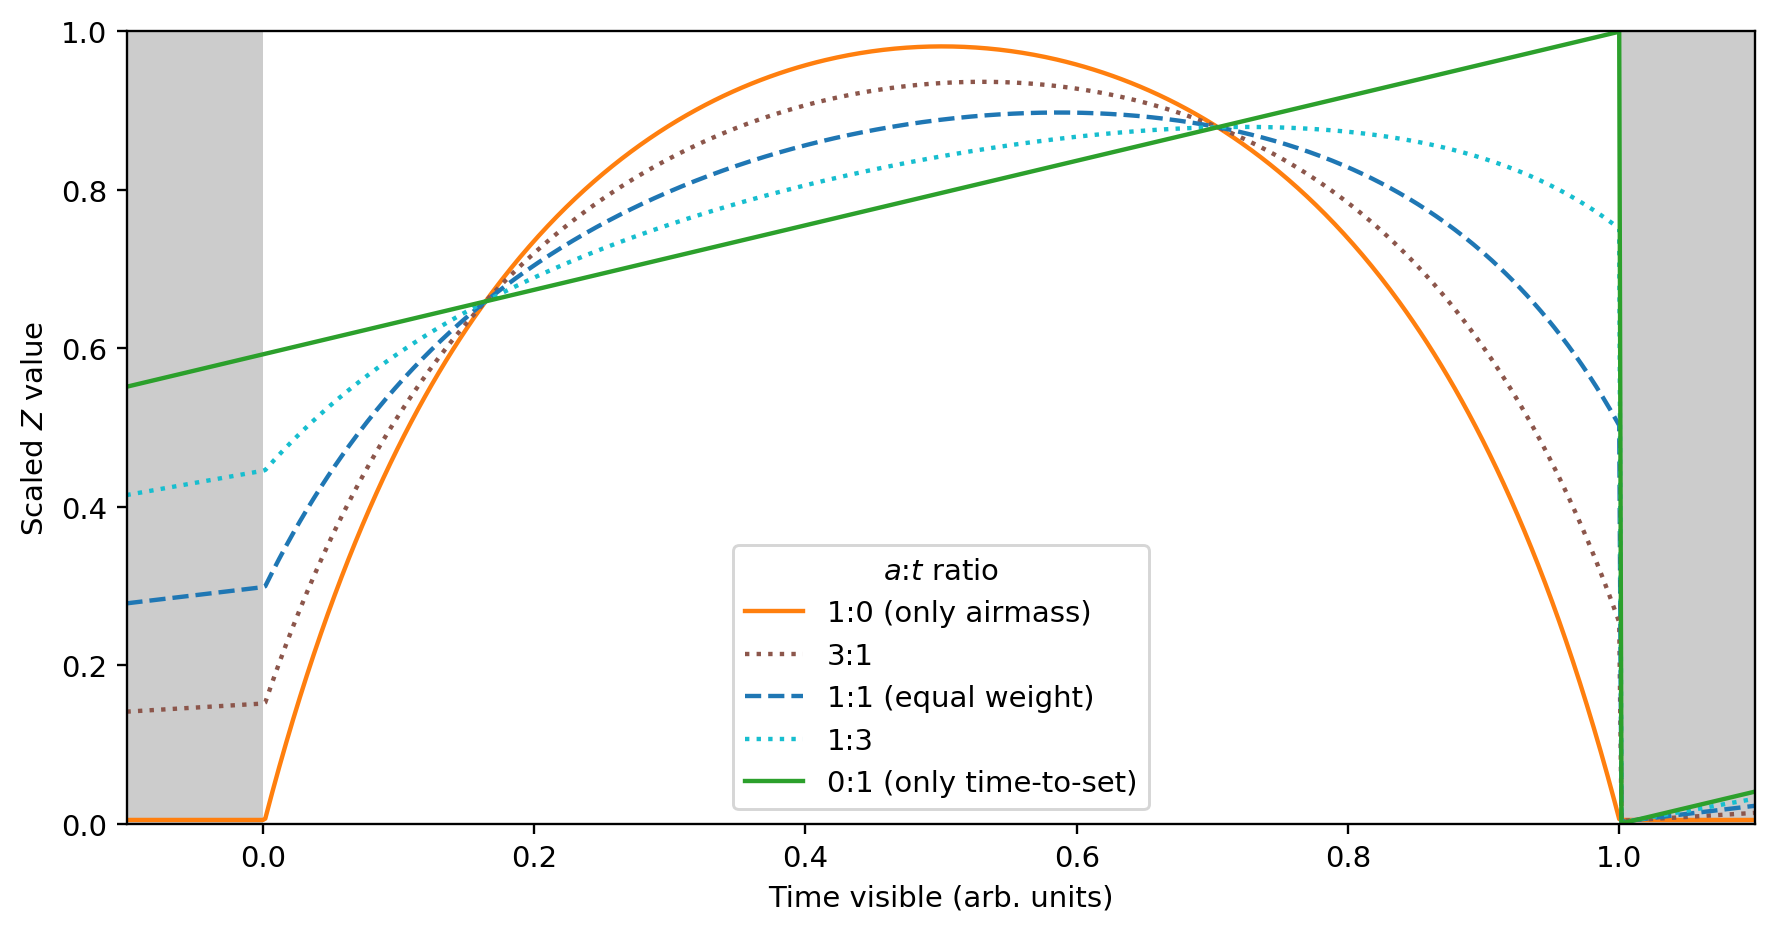
\includegraphics[width=\linewidth]{images/at_ratio.png}
    \end{center}
    \caption[Combining airmass and time-to-set with different ratios]{
        Combining airmass and time-to-set with different ratios. Increasing the relative weighting towards time-to-set shifts the peak of the overall distribution to the right.
    }\label{fig:at_ratio}
\end{figure}

\clearpage

% ---------
\subsubsection{The PAT ratio}

The previous sections detail three different parameters to be considered as part of the scheduler tiebreak parameter: the contained tile probability ($P$), the airmass ($X$) and time-to-set ($T$). Combining these parameters will provide a single, weighted value for each tile at the scheduler check time as

\begin{equation}
    \text{Tiebreak parameter} = \frac{p}{p+a+t} P + \frac{a}{p+a+t} X + \frac{t}{p+a+t} T.
    \label{eq:pat}
\end{equation}

where $p$, $a$ and $t$ are the weightings for the probability, airmass and time-to-set respectively. Together these are called the PAT ratio, and are usually written in the form $p$:$a$:$t$. So a PAT ratio of 1:1:1 means all three are weighted equally, where as 2:1:1 means probability is weighted twice as much as airmass or time-to-set.

\end{colsection}

% ~~~~~~~~~~~~~~~~~~~~


\subsection{Simulation results}
\label{sec:scheduler_sim_results}
\begin{colsection}

A series of simulations were carried out in order to find optimal values for the PAT ratio, and see how the telescope response changes depending on the ratio used. The fake pilot and scheduler code \rtxt{described in the previous section} was run with a selection of skymaps from the LIGO First Two Years project \citep{First2Years}. The PAT ratio was set within the scheduler code, and the skymaps were then added to the observation database and the fake pilot ran through one night of simulated observations for each.

Two primary metrics were used to judge the effectiveness of the simulations. The first was the fraction of the skymap probability covered during the simulated night of observations, the total contained probability within all the tiles that were observed. The second was the mean airmass of each tile when observed. The average of these two values across all the skymaps for the different PAT ratios simulated are plotted in \aref{fig:scheduler_sim_results}.

\begin{figure}[t]
    \begin{center}
        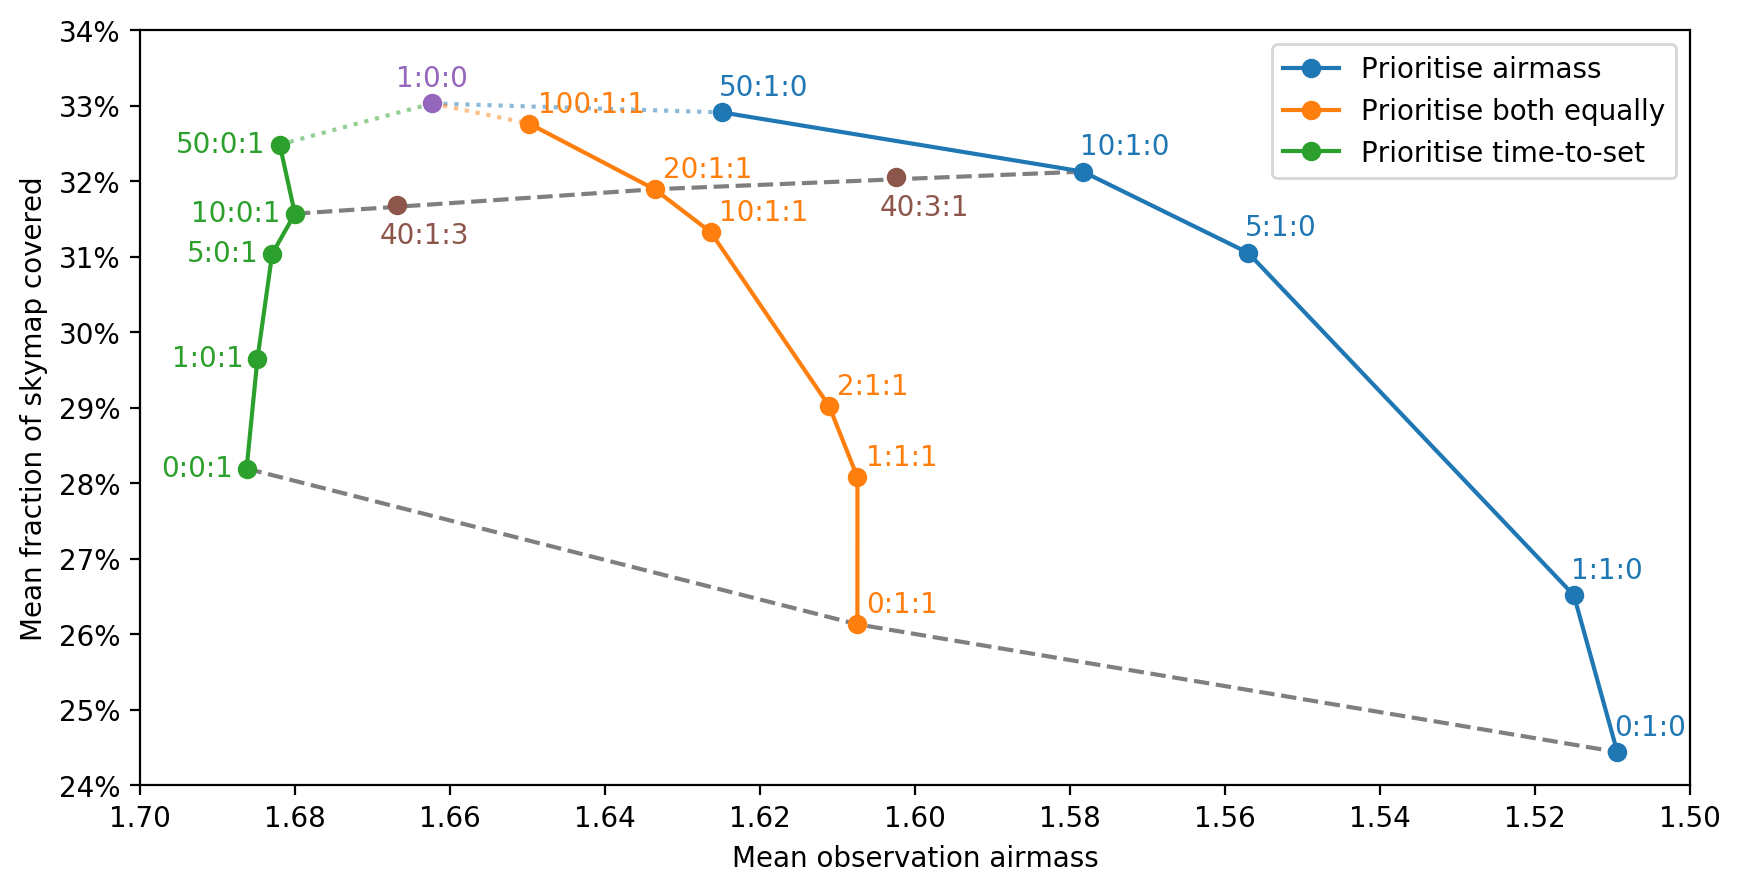
\includegraphics[width=\linewidth]{images/scheduler_sim.png}
    \end{center}
    \caption[Airmass vs fraction of skymap covered for different scheduler weightings]{
        Mean observation airmass vs fraction of the event skymap covered for different scheduler weightings. The full coloured lines join simulations with common airmass:time-to-set ratios, while the dashed lines show some simulations with the same probability weighting relative to the other two parameters. The region formed by the 1:0:0, 0:1:0 and 0:0:1 points contains all possible ratios. The optimal target is low airmass and high fraction covered, corresponding to the top-right of these axes.
    }\label{fig:scheduler_sim_results}
\end{figure}

\end{colsection}

% ~~~~~~~~~~~~~~~~~~~~

\subsection{Analysis of simulation results}
\label{sec:scheduler_sim_analysis}
\begin{colsection}

\aref{fig:scheduler_sim_results} shows several clear trends that emerge from modifying the PAT ratios. Increasing the relative weighting of probability compared to the other two parameters (from 0:X:X, 1:X:X, 5:X:X up to 1:0:0 which is effectively $\infty$:X:X) increases the mean probability covered by up to a third, from 24\% to 33\%. This however typically comes at a cost to the mean airmass of the observations.

Changing the relative ratios of airmass to time-to-set (from Y:1:0 to Y:0:1) shows an unexpected result. It is true the observed airmasses would be lower as less weight is put on the airmass parameter, however it was intended that introducing the time-to-set parameter would compensate by catching more setting tiles that would be missed purely looking around the zenith. This is the result if probability is not included as a factor, as seen by the 0:0:1--1:0:0 line at the bottom of \aref{fig:scheduler_sim_results}. When only airmass is considered (in the 0:1:0 case) the results produce the best average airmass per observation but the worse skymap coverage. On the other hand only considering time-to-set (0:0:1) results in worse airmasses but better coverage. But having the explicit probability parameter counteracts this trend. Looking at the 10:0:1--10:1:0 line changing the airmass to time-to-set ratio only reduces the mean airmass with no corresponding gain in probability covered. In the case where the airmass parameter is ignored (the green time-to-set line on the left of \aref{fig:scheduler_sim_results}) the inclusion of the time-to-set value is just actively suppressing the amount of probability observed while making almost no difference to the mean airmass.

Based on these results, it is clear that the optimal solution is to ignore time-to-set and chose a tiebreaker PAT ratio of around 5:1:0 to 10:1:0, to get the best airmass while limiting the coverage lost. The final scheduler has been operating with a ratio of 10:1:0, as compared to 5:1:0 this gives a gain in mean airmass only 0.02 airmass while increasing the skymap coverage by 1\%. This is only restricting the options to the ratios simulated however, and further simulations would be able to explore the parameter space further.

The results plotted in \aref{fig:scheduler_sim_results} show remarkably smooth trends. The three coloured lines with fixed airmass:time-to-set ratio all curve and trend towards the 1:0:0 point, aside from the slightly outlying 50:0:1 point. The points with a fixed probability weight compared to the other two also seem to form straight lines, as shown by the 10:0:1 to 10:1:0 line. As only the relative values of the ratios matter the 20:1:1 point could be considered to be 10:\sfrac{1}{2}:\sfrac{1}{2}, likewise 40:1:3 and 40:3:1 are 10:\sfrac{1}{4}:\sfrac{3}{4} and 10:\sfrac{3}{4}:\sfrac{1}{4}, from this it is clear that any ratio of airmass to time-to-set will fall on this line if together they add to one-tenth of the probability weighting. However the results shown in \aref{fig:scheduler_sim_results} should be taken with caution. As each point is based on the means over multiply skymaps there is a wide range of variation, and in fact were error bars be included they would have spread off the page in both axes.

The conclusions on the PAT ratio made above are not unreasonable if all that is needed is a one-size-fits-all set of values that are hard-coded into the scheduler, as the current system does use. However when these simulations are revisited it would be a good idea to look more in detail at other trends that might be hidden in the averages. For example if one ratio might be better suited for large skymaps vs smaller ones, or in cases where the whole skymap is visible at once compared to it slowly rising up during the night. These simulations also only considered visibility from La Palma and observed for just the first night, rather than the full 24 hours as used by simulations described later.

These simulations were carried out as the scheduler was still being designed, and long before any of the sentinel or GOTO-alert functions described in \aref{sec:gotoalert} were written. The simulations used the original GOTO-tile code written by Evert Rol to split the skymaps up into the grid, and the individual pointings then had to be added separately into the database. The process in general was a lot slower and required manual intervention to reset the database and ratio values, which is why it took longer to run and fewer simulations were run compared to those described later in this chapter. This was also before GOTO construction began on La Palma, and so properties like the field of view and horizon had to be assumed. Repeating these simulations with the newer code is needed to see if the conclusion that 10:1:0 is still the best case, and at the same time examine the possibility of modifying the ratio based on properties such as the extent of the skymap and time of the event.

Finally, other possible values could be considered for inclusion in the ``PAT'' ratio. One suggestion is to modify time-to-set into time-visible, by including not only the time when the target sets below the horizon but also the time that the Sun rises. The existing time-to-set ratio prioritises observing targets later in the night when they are about to set, where as airmass prioritises tiles near the zenith. Neither however considers the time remaining in the night, and while this is obviously the same for every target it would be better for the time-to-set distribution to peak before sunset instead of after to best prioritise observations in the limted time available.

\end{colsection}

% ~~~~~~~~~~~~~~~~~~~~

\end{colsection}

% ########################################

\newpage
\section{Simulating multiple telescopes and sites}
\label{sec:multi_site}
\begin{colsection}

% ~~~~~~~~~~~~~~~~~~~~

\begin{colsection}

As outlined in Section~\ref{sec:gtecs_multisite} it is envisioned that, as GOTO expands to multiple telescopes and sites, the \gls{gtecs} scheduling system will be extended so that all the telescopes query a single observation database and a master scheduler decides what each telescope should be observing at a given time. This will require a large amount of work to modify both the database structure and the scheduling functions, and as it is not currently implemented into the existing scheduler several workarounds needed to be used in order to create realistic multi-telescope simulations.

\end{colsection}

% ~~~~~~~~~~~~~~~~~~~~

\subsection{Scheduling for multiple observing telescopes}
\label{sec:multi_tel_scheduling}
\begin{colsection}

One of the current restrictions in the scheduling functions (as described in Section~\ref{sec:scheduler}) is that they only ever expect a single Pointing in the observing database to be marked as \code{running} at any one time. It is explicitly coded into the scheduler that detecting multiple running pointings should raise a critical error, as certain bugs early in development could lead to this undesired state to occur. Obviously once the system is to be expanded to multiple telescopes this restriction will have to be lifted, but for these simulations a simplification was required to work around this restriction.

It is currently planned that each telescope will have its own pilot and hardware daemons completely independent of each other, with the only point of overlap being the shared scheduler (and, most likely, the conditions daemon). This makes the master scheduler even harder to consider, as each pilot will be querying it completely out-of-sync. If telescope 1 has just finished observing and makes a scheduler check the scheduler will need to know what telescope 2 is observing, so as not to return the same pointing to telescope 1 (although in some cases having both telescopes observe the same target might be desired, this adds yet another level of complexity). But should both telescopes finish observing at the same time then the scheduler will need some way to decide which gets what target, perhaps deciding by slew time from each telescope's current position.

As none of the above was implemented into the existing code a simplified system was required for these simulations. The existing fake pilot code (\rtxt{described in the previous section}) already contains calls to the real scheduling functions, which return the highest pointing at given time. The simple modification was to make the function return the top $N$ highest pointings, where $N$ is the number of currently observing telescopes. In lieu of any better algorithm to decide which telescope observes which the code simply gives the highest priority pointing to telescope 1, the second highest to telescope 2 and so on. Should there only be one valid pointing returned then only telescope 1 will observe, while telescope 2 will remain ``parked'' until it is needed (this was relevant for the gravitational wave simulations, in practice the second telescope would default to observing the all-sky survey until it also has something to do).

The second simplification was to ensure the telescopes always stayed in sync when observing. The was doable because for either scenario (all-sky survey or \gls{gw} follow-up) each of the pointing would have identical exposure times and therefore take the same amount of time to observe. As there is no need to include simulation steps while the cameras would be exposing the simulation simply increased the time until the observations would be completed. In practice each telescope would take a different amount of time to slew to its target and so quickly get out of sync. Slew time is included in the fake pilot code, from each telescope to its new target. However in order to remain synchronised the code waits the required amount of time for both telescopes to slew and finish their observations. This also accounts for the multiple-running-pointings issue, as by modifying the simulation steps to skip over the actual observing time the pointings never actually need to be marked as \code{running} in the database --- simply going from \code{pending} to \code{completed}. The real observing database would also need a way to record which pointing was observed by which telescope, but that is stored within the fake pilot so there was no need to modify the database schema.

\end{colsection}

% ~~~~~~~~~~~~~~~~~~~~

\subsection{Scheduling for multiple observing sites}
\label{sec:multi_site_scheduling}
\begin{colsection}

The above system provides a good approximation of the response of an arbitrary number of telescopes observing at one site. However expanding the code further to simulate observations from multiple sites adds further complexity.

The scheduler needs to know which site observations are being made from, because it takes into account horizon visibility and airmass. That's simple to include if you have only one site observing at once, but once there are telescopes at multiple sites querying the scheduler at the same time then the responses will need to take that into account. For example, with two telescopes at two sites observing at once the scheduler would need to return the top two pointings at each site, as discussed above. However if the visible portions of the sky from both sites overlap then it's very possible that the same pointing could be the highest priority from both sites. The scheduler would have to chose which of the four telescopes to assign that pointing to, most likely based on the airmass at each site or the slew time from the current target. But then the site that didn't get that pointing assigned now only has the one remaining target to share between its two telescopes. In practice this would mean when querying the scheduler it would have to return the top $X$ pointings, where $X = N_\text{site1} + N_\text{site2} + \cdots$ is the total number of telescopes across the globe (for this example $X=4$).

\begin{figure}[t]
    \begin{center}
        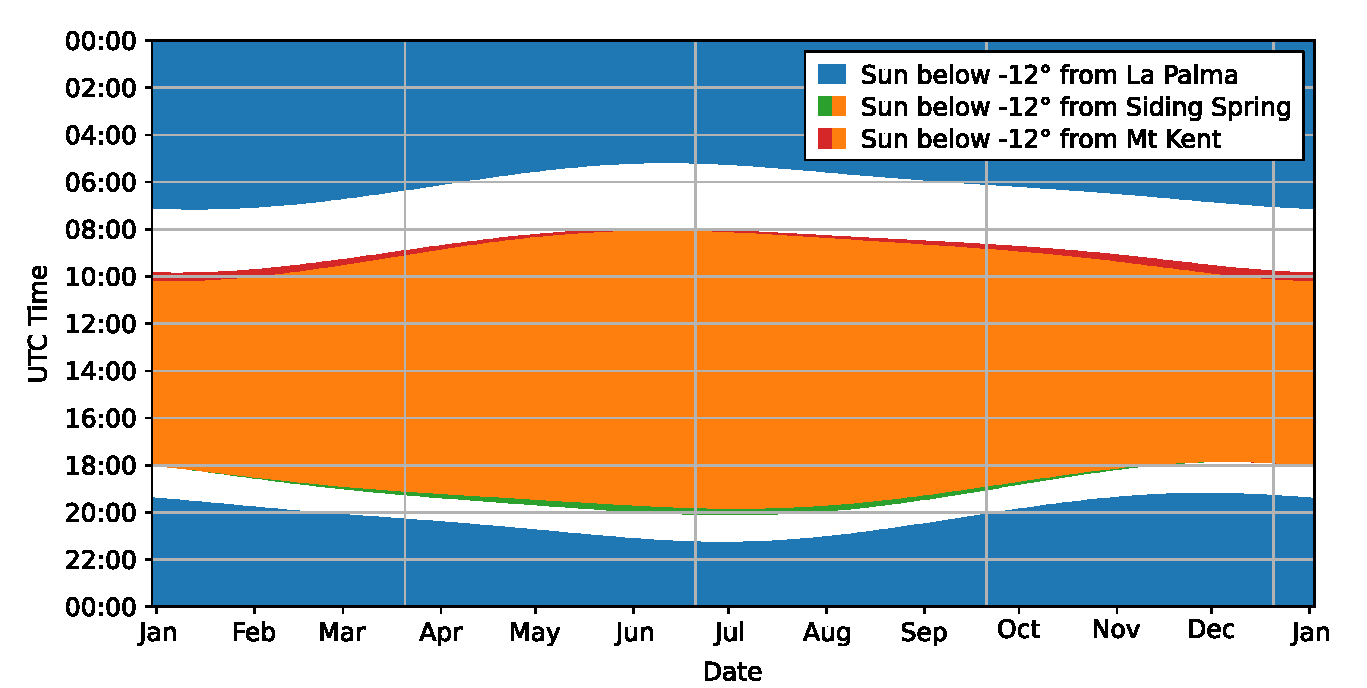
\includegraphics[width=\linewidth]{images/nights.pdf}
    \end{center}

    \caption[Night times throughout the year for GOTO sites]{
        Night times throughout the year for GOTO sites. Night here is defined as when the Sun is \SI{12}{\degree} below the local horizon.
    }\label{fig:nights}
\end{figure}

The above system would be possible to implement in the simulations, but there is a lucky simplification that can be made for the specific cases that are being considered. Saying the scheduler needs to find the top $X$ pointings, where $X$ is the total number of telescopes at all sites, is not strictly true --- it actually only needs to return enough pointings to satisfy the telescopes at the sites that are currently observing. In other words it there are two sites but one is shut down, due to weather or because it is daytime there, the scheduler doesn't need to worry about choosing which site pointings are assigned to as only the one is currently active. Conveniently for simulating the proposed GOTO network this is always true: using a horizon of \SI{-12}{\degree} the periods of darkness between La Palma and either of the Australian sites never overlap. This is shown in Figure~\ref{fig:nights}, where there is a constant ``buffer zone'' between night ending at one site and beginning at the other. This case only applies for a very limited number of combinations of sites. As shown in Figure~\ref{fig:site_nights} there is a tear-drop-shaped area on the Earth's surface which contain the locations where the local night will never overlap with night on La Palma, comprising only of eastern Australia, New Zealand and Melanesia. For a horizon of \SI{-12}{\degree} this area contains just $6.6 \%$ of the Earth's surface.

The convenient location of the Australian sites means implementing them into the simulation code was fairly simple. Should simulations for other sites on the Earth be included that aren't within the small non-overlapping area, for example other backup GOTO-South sites in South Africa or Chile, the code would need to be expanded as described above. In principle the simulations can be run for any one site on the Earth as a stand-alone observatory, and then this could be combined afterwards with the results from other, stand-alone simulations. This however removes the benefit of the sites acting together and using a common observing database. Section~\ref{sec:gw_sims} considers this in more detail for sites with different grids.

\begin{figure}[p]
    \begin{center}
        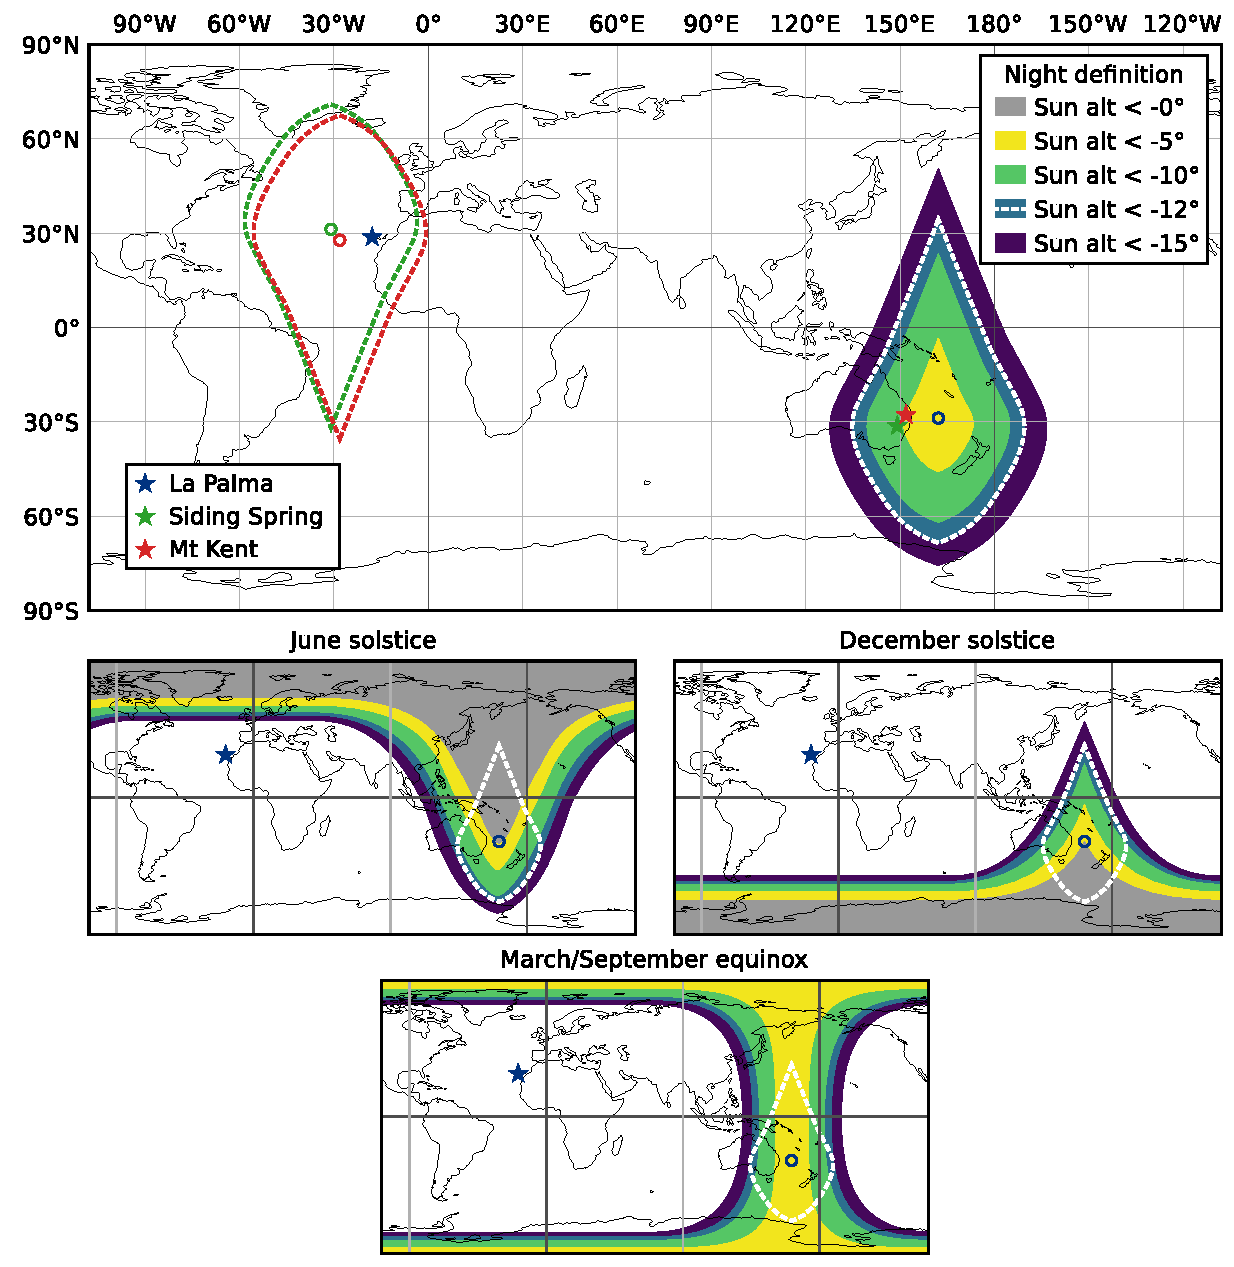
\includegraphics[width=\linewidth]{images/sites.pdf}
    \end{center}

    \caption[Locations on the Earth with non-overlapping night times]{
        Finding locations on the Earth with non-overlapping night times. On the upper plot the filled areas show the locations on the Earth where local night never overlaps with night on La Palma, at any point in the year. The different colours denote different horizon definitions, with the \SI{-12}{\degree} horizon also being surrounded by a white dashed line. The location of the GOTO sites considered (\textcolor{blue}{La Palma}, \textcolor{ForestGreen}{Siding Spring} and \textcolor{red}{Mt Kent}) are marked with stars and their antipodes are marked with hollow circles. The equivalent areas for Siding Spring and Mt Kent are also shown by the coloured dashed lines surrounding their antipodes, for a \SI{-12}{\degree} horizon only. The lower plots shows how the region varies over a year, from the solstices via the equinox (the plot is identical for the March and September equinoxes and therefore is only shown once).
    }\label{fig:site_nights}
\end{figure}

\clearpage

\end{colsection}

% ~~~~~~~~~~~~~~~~~~~~

\subsection{Simulating different grids}
\label{sec:multi_grid_scheduling}
\begin{colsection}

One fundamental feature of the existing \gls{goto} code is that observations are carried out on an all-sky grid, as defined in Section~\ref{sec:gototile}. When considering multiple telescopes this is both useful in some ways and limiting in others. Having a fixed grid that is common to all telescopes is vital for the \gls{goto} image subtraction systems, which is why it is anticipated to form the base of the global system. By sharing tiles each telescope can contribute to the same all-sky survey grid, as well as coordinate mapping out a gravitational wave skymap.

However sharing the grid requires all the telescopes to have essentially the same field of view. There is some leeway in the exact field of view of each array, tiles in the existing grid are not defined to cover precisely the combined output of all the telescopes but leave a slight overlap around the edge (\rtxt{see figure in commissioning}). But if the field of view is much larger than the tile tile size then the pointings will be too close together and therefore inefficient. Worse is if the field of view is much smaller than the defined tile size, as it would lead to gaps on the sky between observations.

For the proposed \gls{goto} system with near-identical \gls{goto}-8 units around the world this is not an issue, but it should be recognised as a limitation of not just the simulations but the whole \gls{gtecs} control system. One potential case where this may be an issue is when commissioning \gls{goto}-South. If it spends time as a GOTO-4 system similar to La Palma before getting the second set of unit telescopes then it will be observing concurrently with one or two GOTO-8 systems on La Palma. This is a likely enough situation that it was considered in the gravitational wave simulations as described in Section~\ref{sec:gw_sims}, using the work around of two independent simulations as mentioned above. How this set-up would be dealt with within a real implementation of \gls{gtecs} is a problem that needs development in the future should it prove to be necessary.

\end{colsection}

% ~~~~~~~~~~~~~~~~~~~~

\end{colsection}

% ########################################

\newpage
\section{Gravitational wave follow-up simulations}
\label{sec:gw_sims}
\begin{colsection}

% ~~~~~~~~~~~~~~~~~~~~

\begin{colsection}

As the primary mission of the \gls{goto} project is to follow up gravitational wave detections, it is important to consider what benefit additional telescopes will bring to the project. In order to do this, simulations were run on the LIGO First Two Years mock skymaps \citep{First2Years}. The sample contained 1105 events, each based on simulating a binary neutron star coalescence at a particular sky position and distance. Each event had two skymaps generated: the first using the rapid \code{BAYESTAR} pipeline, which is typically available minutes after the event, and the second using the \code{LALInference} code which can take hours or days to complete. For these simulations therefore only the \code{BAYESTAR} skymaps were considered in order to focus on \gls{goto}'s initial follow-up, although an extension to the simulations could include the effects of the second updated skymap being processed and added to the database some hours after the event time.

\end{colsection}

% ~~~~~~~~~~~~~~~~~~~~

\subsection{Event visibility}
\label{sec:gw_visability}
\begin{colsection}

The simulations were designed to begin at the time of the event, and then simulate the next 24 hours of observations. This therefore guaranteed one night's worth of observing at each site, although split into two halves if the event occurred during the night. The time each event occurred was taken from the simulated skymaps, as the \citet{First2Years} simulations considered factors such as the duty cycle of each detector maintaining the time was important. Events were uniformly distributed in time of occurrence (at what time during the day), while in date they all occur over a two month period spanning either side of the 2010 September equinox, as shown in \aref{fig:f2y_times}. It is not clear why this range of dates was selected, although surrounding one of the equinoxes might have been an attempt to reduce bias towards observers from either hemisphere. Detailed analysis shows the events are not entirely equally distributed either side of the equinox (03:09 on 2010--09--23), with the first occurring 33 days before and the second 27 days after. Overall 64\% of events occur before the September equinox and 36\% after, this leads to a slight bias in terms of visibility towards the southern sites as they will experience longer nights before the equinox (in the southern winter).

\begin{figure}[t]
    \begin{center}
        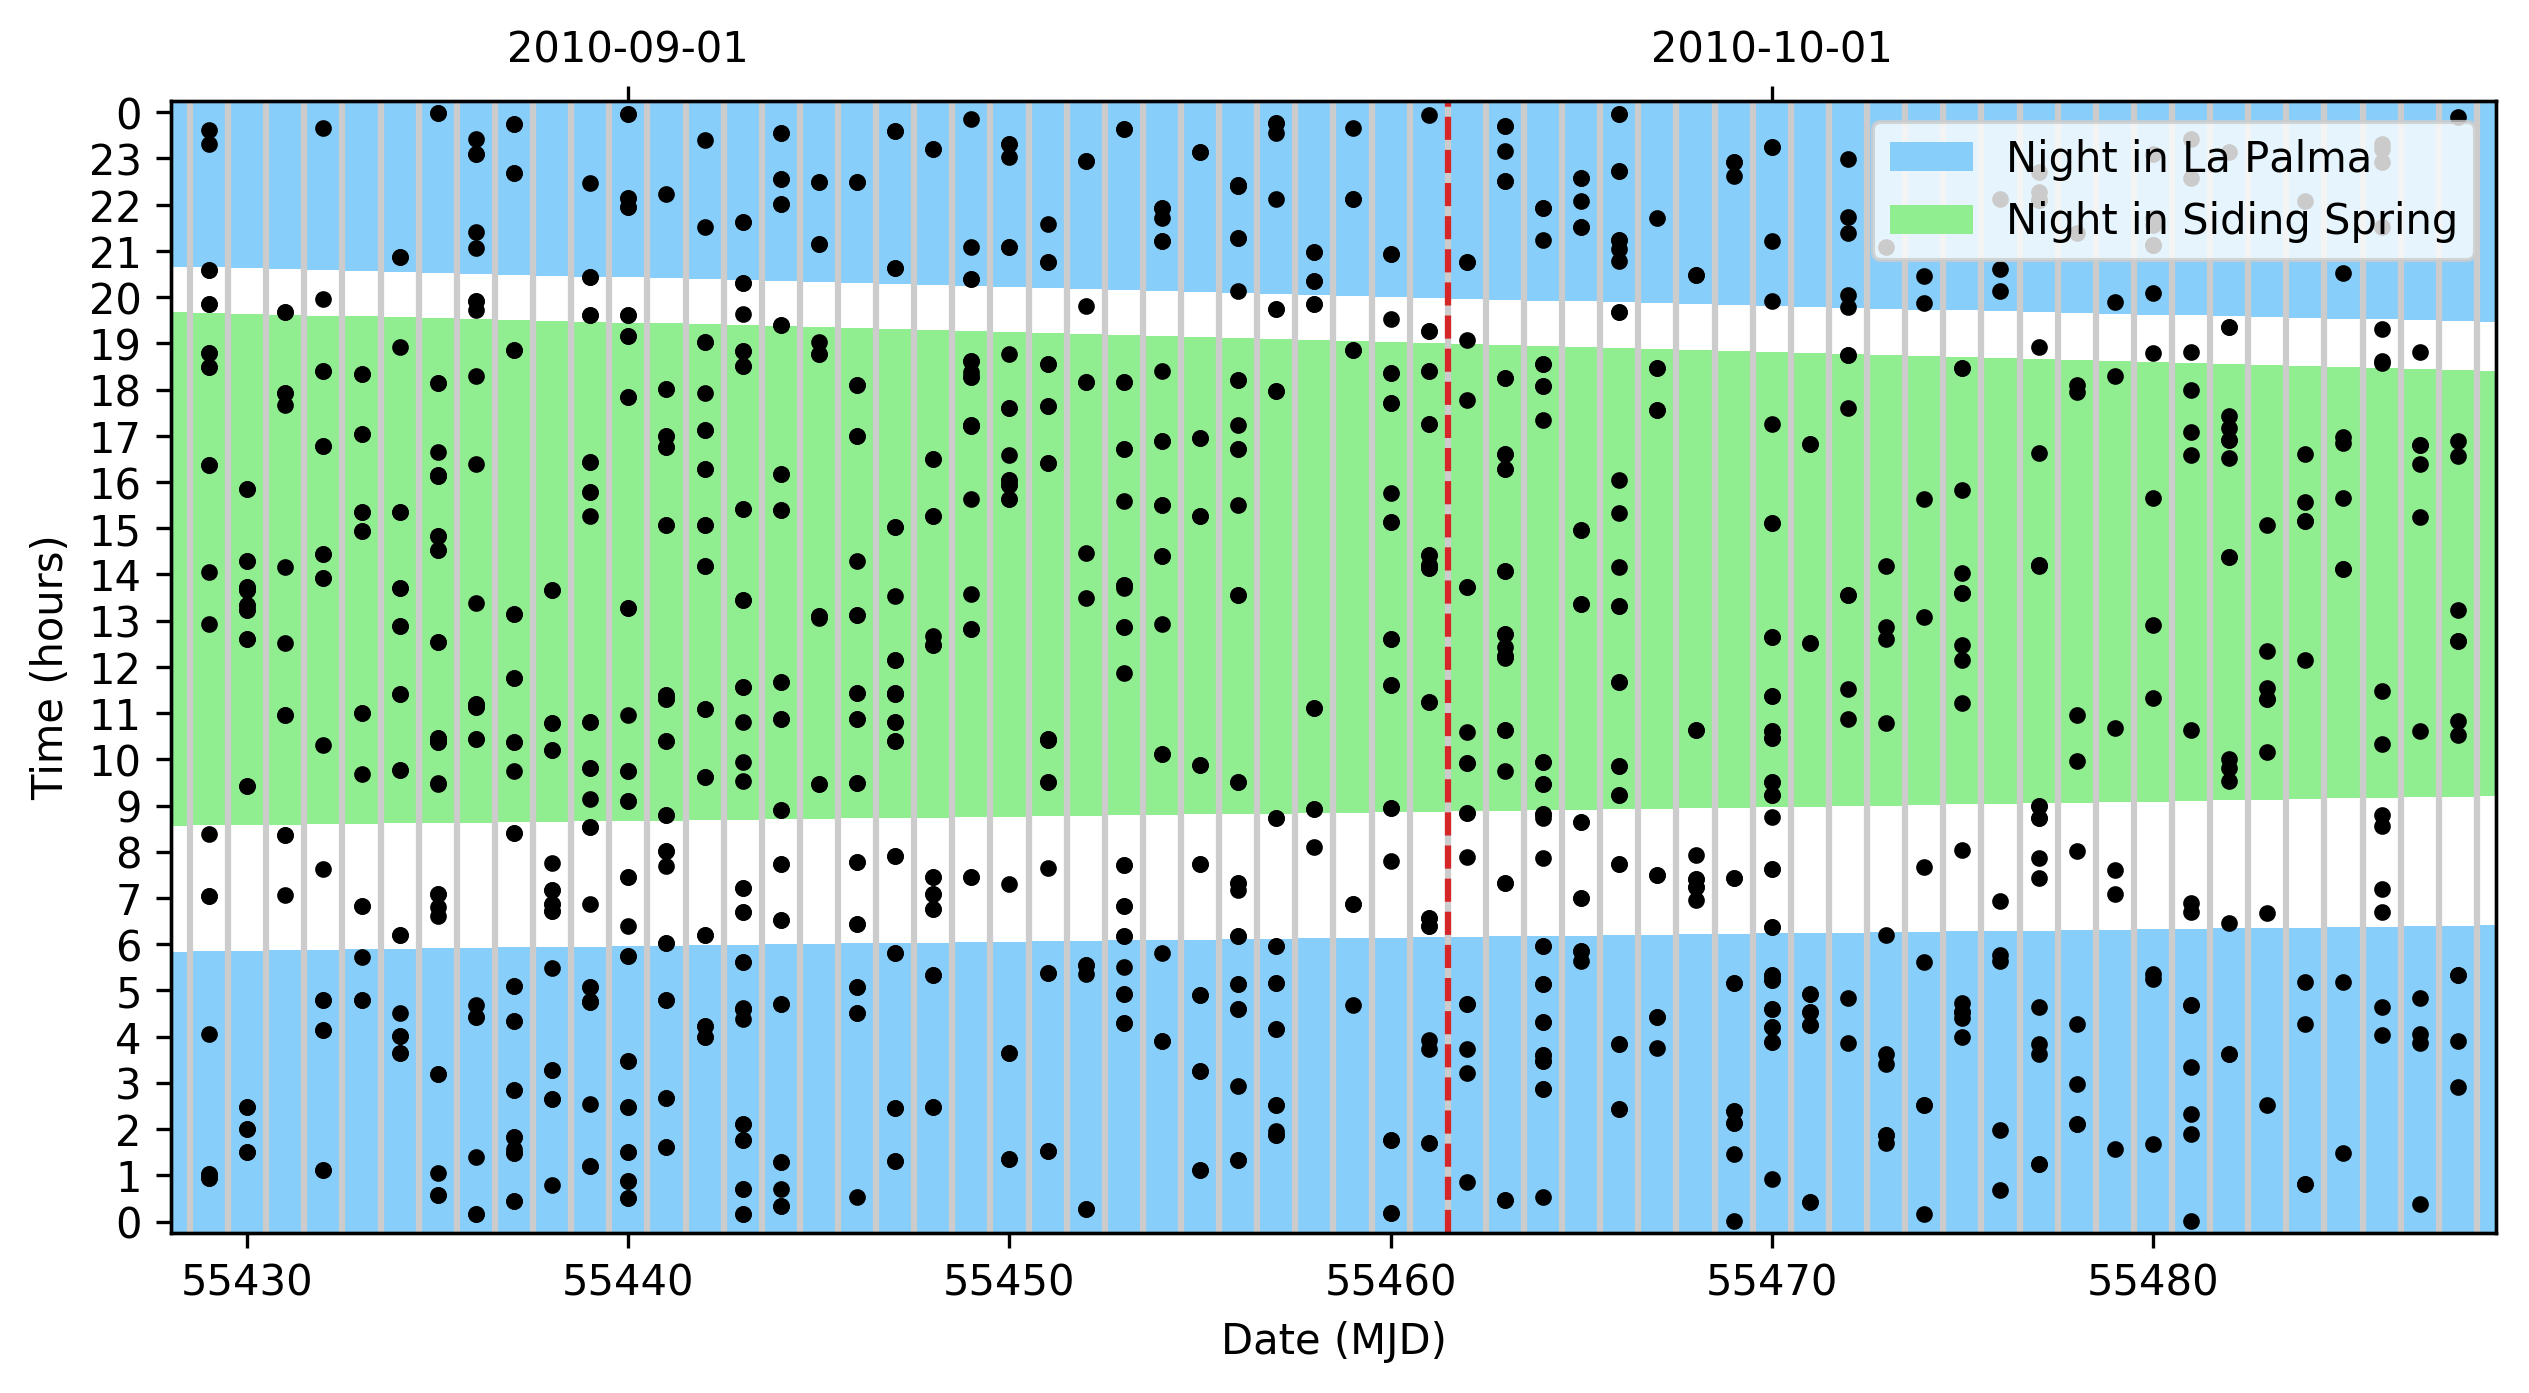
\includegraphics[width=\linewidth]{images/f2y_times.png}
    \end{center}

    \caption[Date and time distribution of events in the First Two Years sample]{
        Date and time distribution of events in the First Two Years sample \citep{First2Years}. The night periods are shown for La Palma and Siding Spring. The equinox is shown by the red dashed line. \rtxt{TODO --- Inkscapify}
    }\label{fig:f2y_times}
\end{figure}

Events were uniformly distributed across the sky, and are uniform in distance cubed. Although each source included distance information this was not taken into account in the simulations aside from determining the event strategy to use (all were well within the \SI{400}{\mega\parsec} definition for close neutron star events defined for GOTO-alert in \aref{sec:event_strategy}). Future simulations could use the distance to the event to estimate a light curve based on that of GW170817 and use it to predict how long each event would be visible for. As GW170817 only faded below \gls{goto}'s 20 mag limit after 2.5 days a 24 hour period is a reasonable amount of time to simulate.

The first stage of the simulations was to determine if the event source was going to be physically visible from the considered sites in the 24 hours after the event occurred. In order to save time it decided to not spend time running full fake pilot simulations for events which would never be observed, and therefore the simulation for that event was aborted early if no tiles that the source was located within were going to be visible. Each event was classified into one of four categories:

\begin{itemize}
    \item \textbf{Not visible --- too close to the Sun}. These events had sources that were too close to the Sun within the 24 hour period to observe. This was defined as being within \SI{42}{\degree} of the Sun at any point over the 24 hours (\SI{12}{\degree} from the definition of night time plus \SI{30}{\degree} from the horizon limit). This region corresponds to an area of the sky that is not visible from any site on Earth using these observing parameters. It is a fixed fraction of the sky: 5280 sq deg or 13\% of the celestial sphere\footnote{The area of a circle with radius $r$ on the surface of a sphere with radius $R$ is $2\pi R^2(1-\cos(r))$. The radius of the celestial sphere $R=\SI{360}{\degree}/2\pi \approx \SI{57.3}{\degree}$.}.

    \item \textbf{Not visible --- below declination limit}. These event sources fall within the region of the sky that are never visible form a given site due to the limited declination range. For example, using the standard \SI{30}{\degree} horizon limit over the course of a year sa telescope on La Palma (latitude \SI{28}{\degree} N) can see a band of sky between \SI{+88}{\degree} and \SI{-32}{\degree} declination. Sources outside of this region (that are not already excluded due to being too close to the Sun) would therefore never be observable from the given site, but could be observed from other locations. At the equator this band covers 87\% of the sky, at latitudes of $\pm \SI{30}{\degree}$ 75\% of the sky is visible, falling to just 25\% at the poles\footnote{The area of a segment on a sphere between angles $\theta$ and $\phi$ is $2 \pi R^2 (\cos(\theta)-\cos(\phi))$}.

    \item \textbf{Not visible --- event time}. These event sources are outside of the hard Sun limit and within the visible declination range, but are still not observable during the given 24 hour period as they have set by the time the night begins. Like sources below the declination limit, sources located within this region would be visible from other sites at different latitudes.

    \item \textbf{Visible}. The source for this event falls outside of either of the above three areas, and therefore is nominally above the horizon limit at some point during night time within 24 hours after the event. The portion of the sky that is visible in one night from a given site depends on the latitude of the site and the time of year.
\end{itemize}

\begin{table}[t]
    \begin{center}
        \begin{tabular}{c|ccc} % chktex 44
            \multirow{3}{*}{Night} & \multicolumn{3}{c}{Site} \\
                      & La Palma             & Siding Spring  & Mt Kent \\
                      & (\SI{28}{\degree} N) &  (\SI{31}{\degree} S) &  (\SI{27}{\degree} S) \\
                      \midrule
                      \\
            March     & \textcolor{Green}{57.1\% visible}
                      & \textcolor{Green}{56.3\% visible}
                      & \textcolor{Green}{59.6\% visible}
                      \\
            equinox   & {\scriptsize(\textcolor{BurntOrange}{12.9\%} $\cdot$
                                     \textcolor{NavyBlue}{23.4\%} $\cdot$
                                     \textcolor{Blue}{6.7\%})}
                      & {\scriptsize(\textcolor{BurntOrange}{12.9\%} $\cdot$
                                     \textcolor{NavyBlue}{24.6\%} $\cdot$
                                     \textcolor{Blue}{6.2\%})}
                      & {\scriptsize(\textcolor{BurntOrange}{12.9\%} $\cdot$
                                     \textcolor{NavyBlue}{22.5\%} $\cdot$
                                     \textcolor{Blue}{5.0\%})}
                      \\[0.5cm]
            June      & \textcolor{Green}{50.4\% visible}
                      & \textcolor{Green}{61.9\% visible}
                      & \textcolor{Green}{62.7\% visible}
                      \\
            solstice  & {\scriptsize(\textcolor{BurntOrange}{12.9\%} $\cdot$
                                     \textcolor{NavyBlue}{24.2\%} $\cdot$
                                     \textcolor{Blue}{12.4\%})}
                      & {\scriptsize(\textcolor{BurntOrange}{12.9\%} $\cdot$
                                     \textcolor{NavyBlue}{20.9\%} $\cdot$
                                     \textcolor{Blue}{4.3\%})}
                      & {\scriptsize(\textcolor{BurntOrange}{12.9\%} $\cdot$
                                     \textcolor{NavyBlue}{19.0\%} $\cdot$
                                     \textcolor{Blue}{5.4\%})}
                      \\[0.5cm]
            September & \textcolor{Green}{57.0\% visible}
                      & \textcolor{Green}{56.4\% visible}
                      & \textcolor{Green}{57.7\% visible}
                      \\
            equinox   & {\scriptsize(\textcolor{BurntOrange}{12.9\%} $\cdot$
                                     \textcolor{NavyBlue}{23.4\%} $\cdot$
                                     \textcolor{Blue}{6.7\%})}
                      & {\scriptsize(\textcolor{BurntOrange}{12.9\%} $\cdot$
                                     \textcolor{NavyBlue}{24.5\%} $\cdot$
                                     \textcolor{Blue}{6.2\%})}
                      & {\scriptsize(\textcolor{BurntOrange}{12.9\%} $\cdot$
                                     \textcolor{NavyBlue}{22.4\%} $\cdot$
                                     \textcolor{Blue}{7.0\%})}
                      \\[0.5cm]
            December  & \textcolor{Green}{62.5\% visible}
                      & \textcolor{Green}{48.9\% visible}
                      & \textcolor{Green}{51.0\% visible}
                      \\
            solstice  & {\scriptsize(\textcolor{BurntOrange}{12.9\%} $\cdot$
                                     \textcolor{NavyBlue}{19.7\%} $\cdot$
                                     \textcolor{Blue}{4.8\%})}
                      & {\scriptsize(\textcolor{BurntOrange}{12.9\%} $\cdot$
                                     \textcolor{NavyBlue}{25.8\%} $\cdot$
                                     \textcolor{Blue}{12.4\%})}
                      & {\scriptsize(\textcolor{BurntOrange}{12.9\%} $\cdot$
                                     \textcolor{NavyBlue}{23.2\%} $\cdot$
                                     \textcolor{Blue}{12.9\%})}
                      \\
        \end{tabular}
    \end{center}

    \caption[Sky visibility over a year]{
        Sky visibility over a year from the three different \gls{goto} sites. The upper value shows the fraction of the sky that is \textcolor{Green}{visible} within the night. The lower values break down the remaining fraction of the sky into the three non-visible categories (\textcolor{BurntOrange}{too close to the Sun}, \textcolor{NavyBlue}{below declination limit} and \textcolor{Blue}{event time}).
    }\label{tab:visibility}
\end{table}

The region of the sky visible during the night for a given site change over the course of the year. \aref{tab:visibility} shows the fractions of the sky in each of the four categories above at the four solstices and equinoxes during the year. \aref{fig:visibility} plots the regions on the celestial sphere, in order to better visualise how they change depending on observing site and time of year.

\begin{figure}[p]
    \begin{center}
        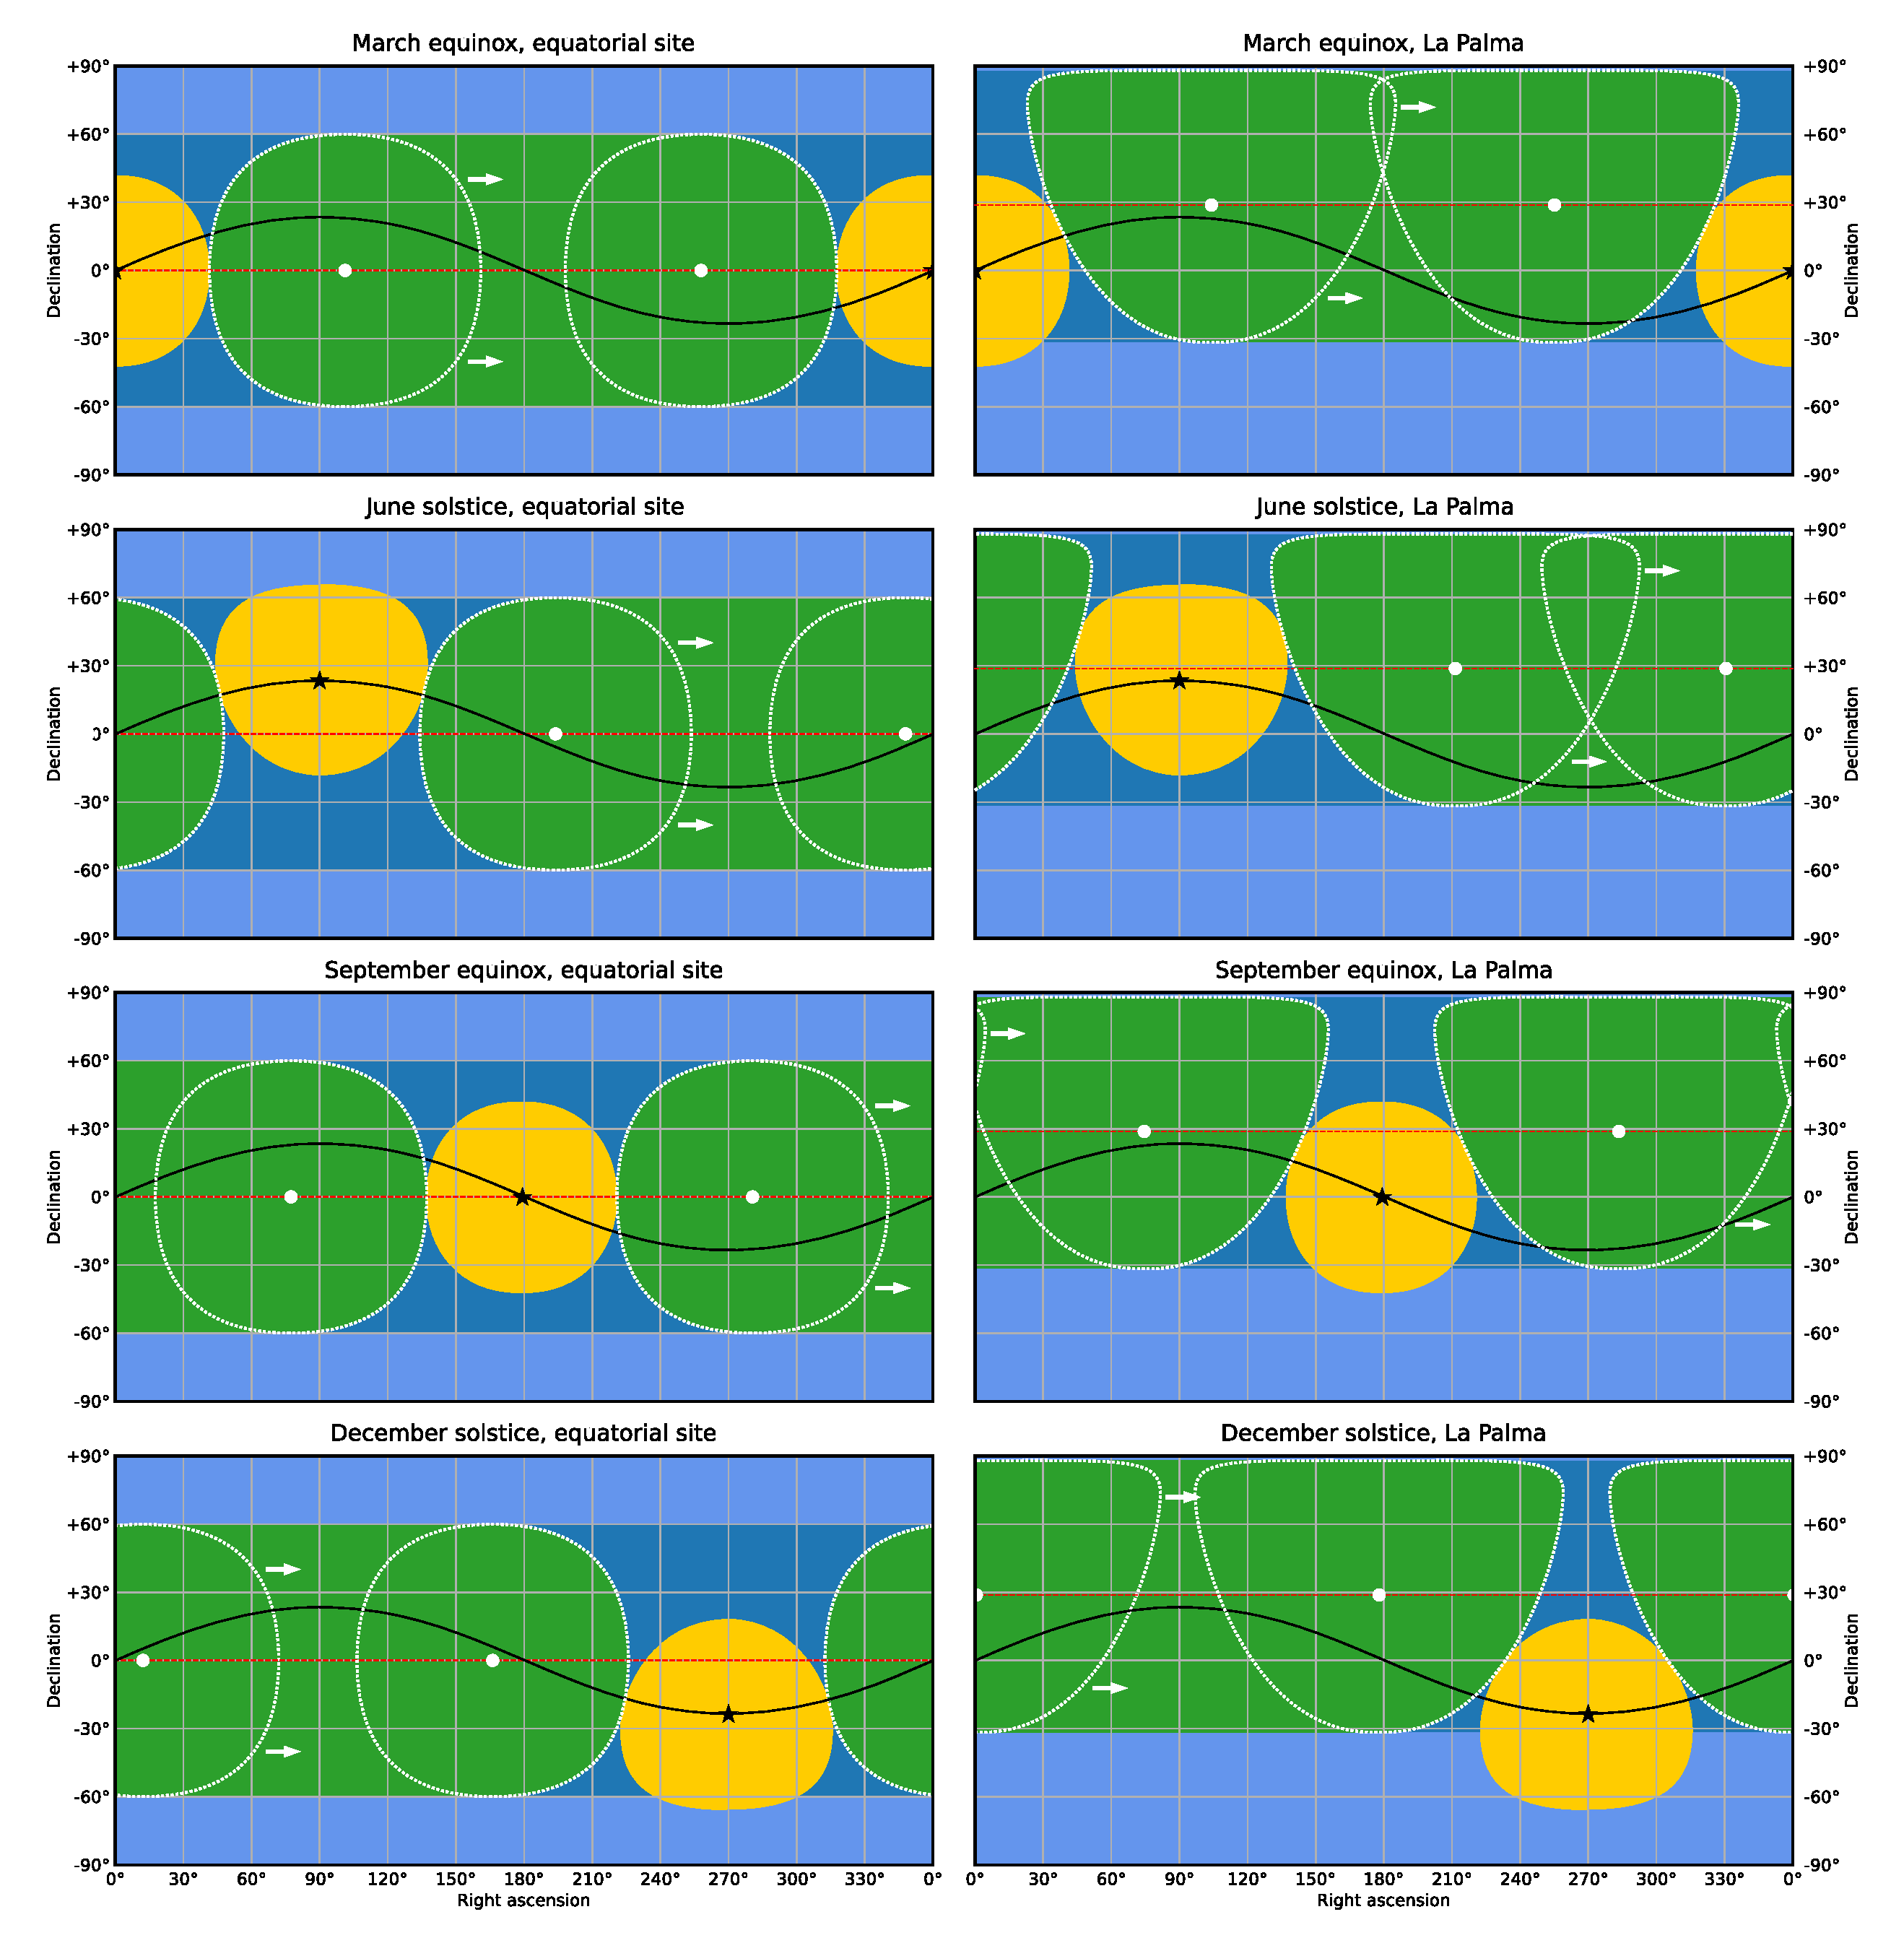
\includegraphics[width=\linewidth]{images/visibility.pdf}
    \end{center}
    \caption[Plotting sky visibility regions over a year]{
        Changing sky visibility regions over a year, plotted on the celestial sphere. The left column shows visibility for a theoretical observer located on the Earth's equator, the right-hand column shows visibility from the latitude of La Palma (\SI{28}{\degree} N). Visibility is plotted for four different nights, at the equinoxes and solstices. Regions in \textcolor{Green}{green} are visible during the night, with the visible portion of the sky at sunrise and sunset denoted by the white dashed lines. Regions in \textcolor{NavyBlue}{light blue} are out of the visible declination range of the site and so are never visible, regions in \textcolor{Blue}{dark blue} would be visible but not during the given night. Finally the \textcolor{BurntOrange}{yellow} area shows the \SI{42}{\degree} region around the Sun that is excluded from any site on Earth. The black line shows the ecliptic, with the black star marking the position of the Sun (the Sun does move slightly along this path during the night but it is not visible at this scale, the star marks the position at local midnight).
    }\label{fig:visibility}
\end{figure}

\clearpage

\end{colsection}

% ~~~~~~~~~~~~~~~~~~~~

\subsection{Selecting event tiles}
\label{sec:gw_selecting}
\begin{colsection}

Even if an event source is visible within the 24 hours from a given site (or combination of sites) there is one further criteria that would prevent observations of the source, that being whether the source is located within any of the tiles added to the database. The issue of determining which tiles to add to the database is detailed in \aref{sec:db_insert}, but is ultimately a matter of probability. If the telescope covered the 90\% confidence region for every event then it would be expected to observe 90\% of the event sources. Two particular examples are shown in \aref{fig:poor_selection}.

GOTO-alert uses the mean contour level method to select tiles as described in \aref{sec:db_insert}, which itself requites further simulations to find an optimal level to use. The level will also need modification based on the tile shape. For these simulations a mean contour selection value of $0.9$ was used for the GOTO-4 grid and $0.95$ for the GOTO-8 grid. Using these values 92\% of events had sources within at least one of the selected tiles for the GOTO-4 grid, and 95\% for the GOTO-8 grid. In the following simulation results the tile selection was considered \textit{after} the visibility restrictions in the previous section, as it is an operational value decided for \gls{goto} while the visibility is true for any and all telescopes at the relevant sites.

Future simulations should be run using the same sample of skymaps but altering the selection level, and comparing the number of selected sources to the number of tiles selected for each event. As discussed in \aref{sec:db_insert} there is a trade-off between adding two few tiles and missing the source and adding too many and increasing the time to cover them all. As additional telescopes are added the limit can also be relaxed further, as they will pass through observing the selected tiles faster.

\begin{figure}[p]
    \begin{center}
        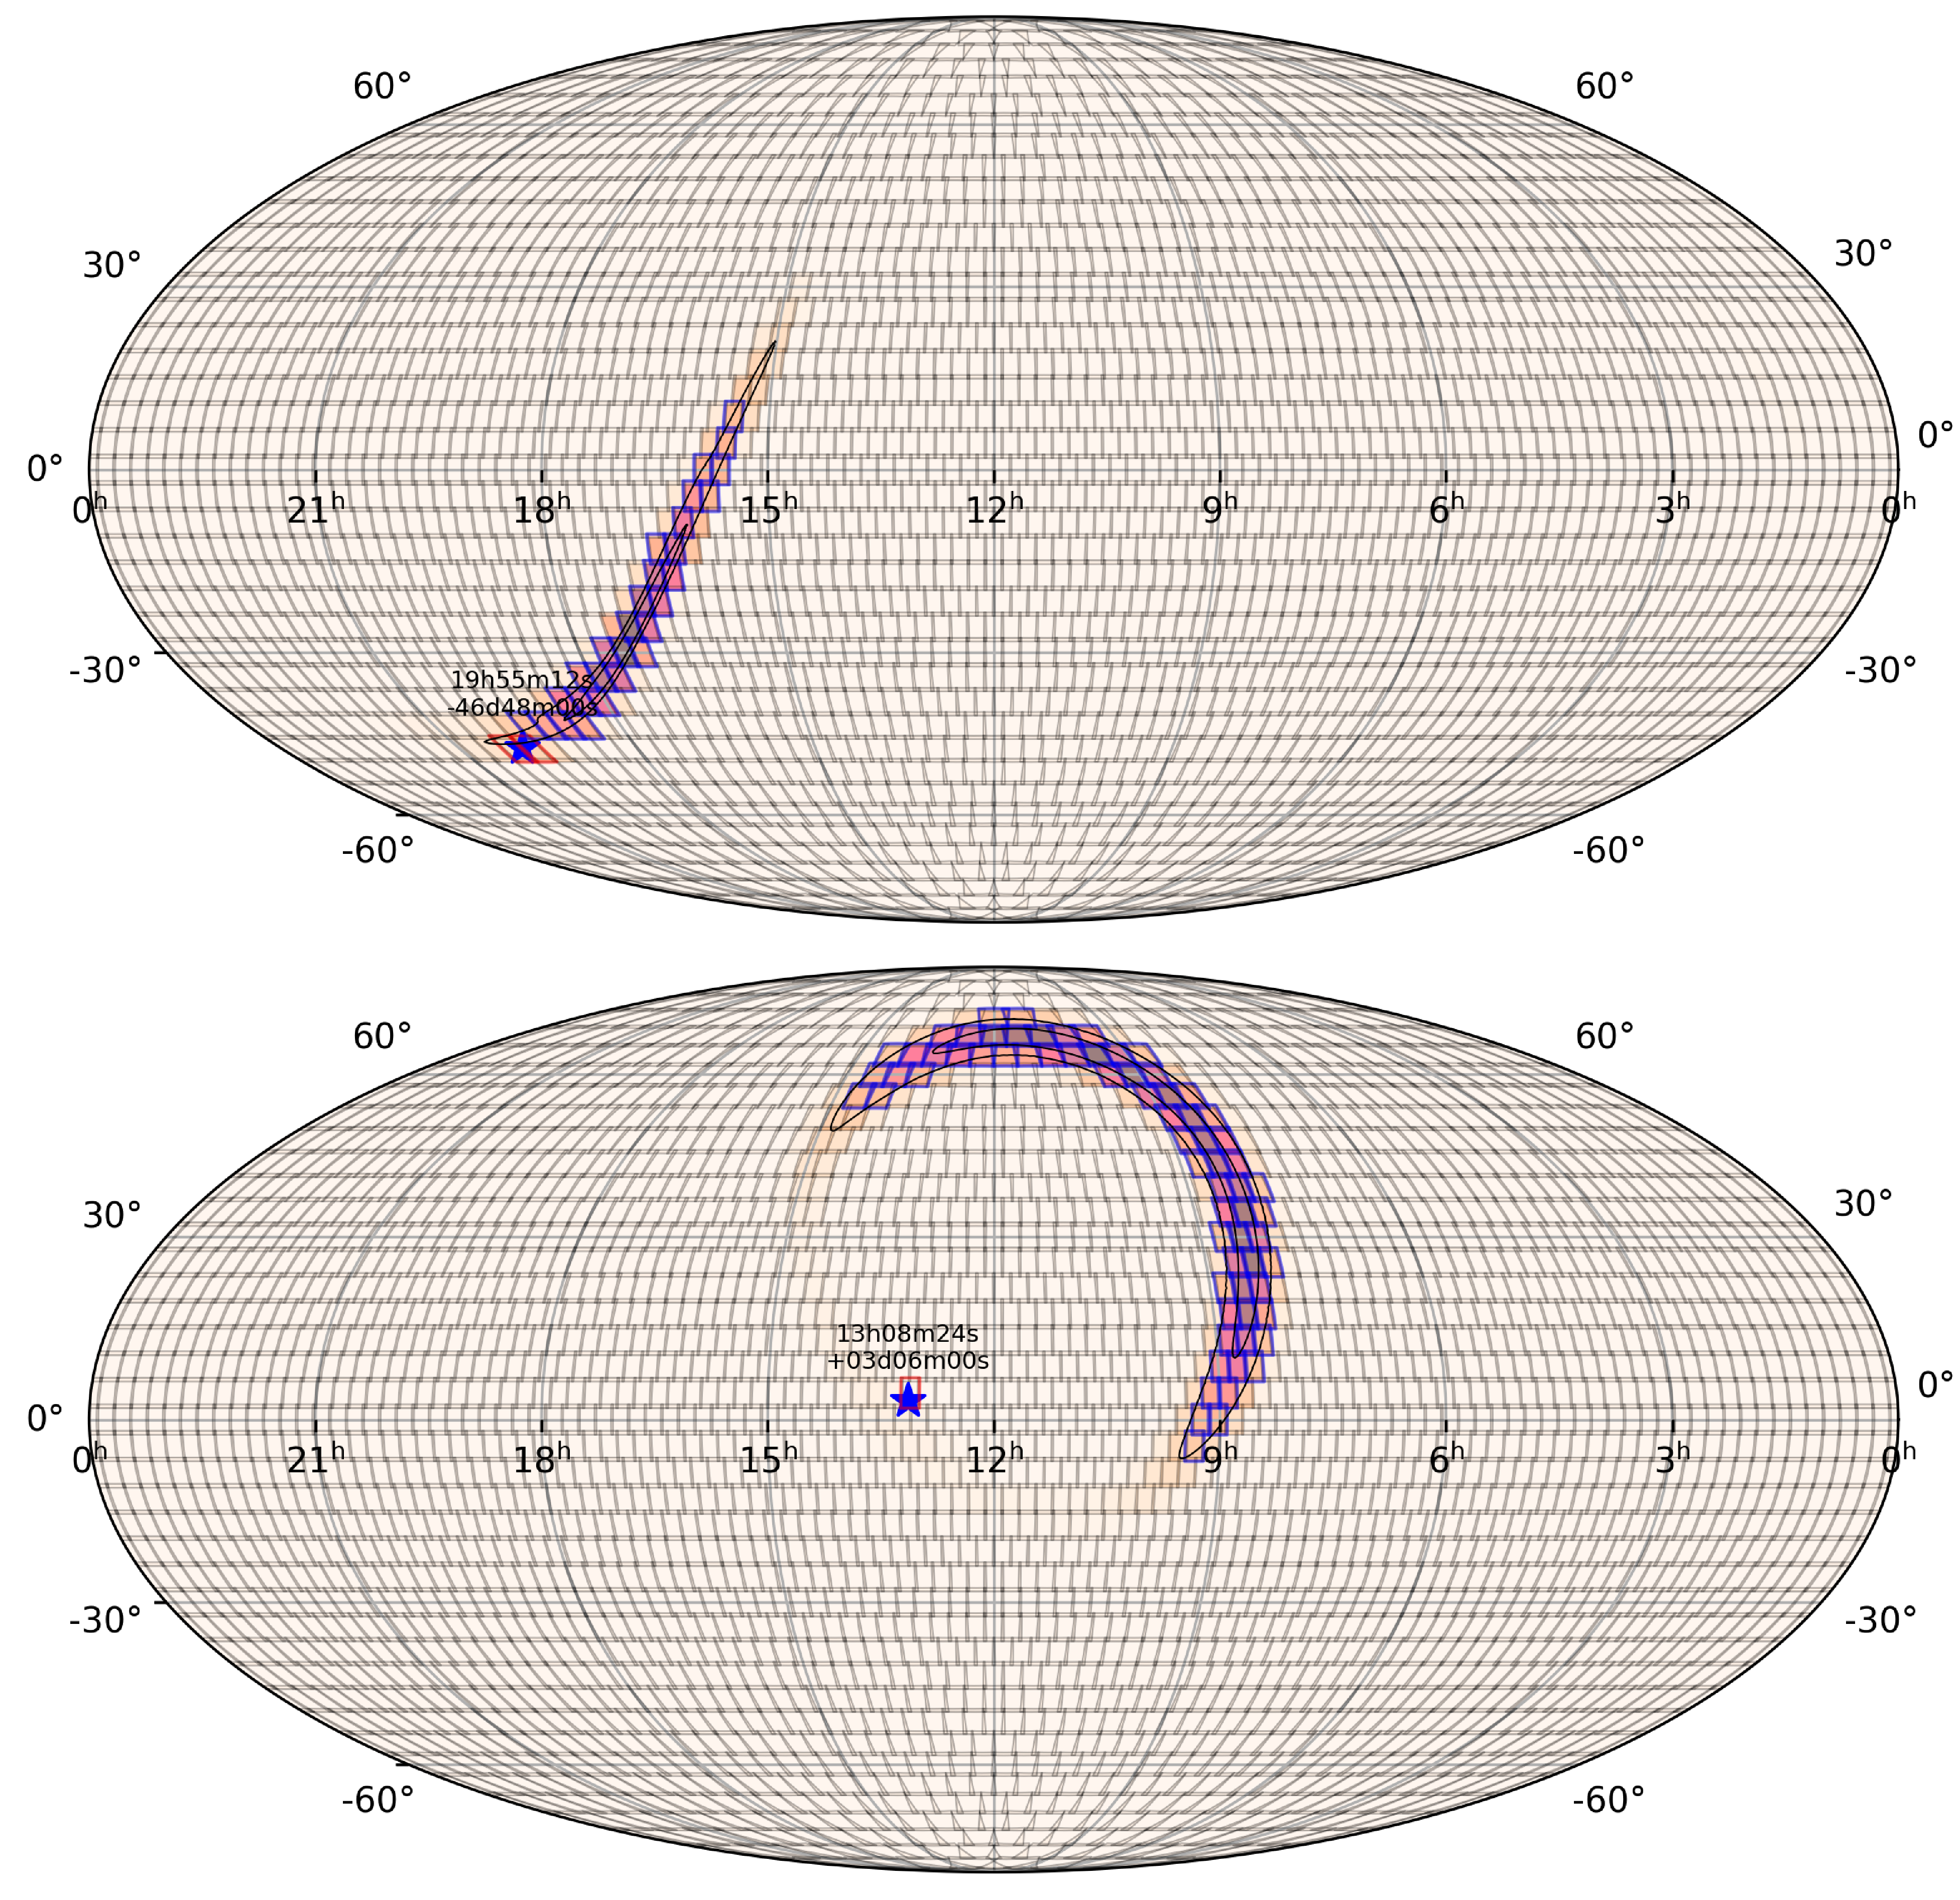
\includegraphics[width=\linewidth]{images/non_selected.pdf}
    \end{center}
    \caption[Examples of mock GW event sources falling outside of the selected tiles]{
        Two examples of mock GW event sources (marked by the blue star) falling outside of the selected tiles (blue highlighted tiles). In the upper case (trigger ID 13630) the tiles the source fell within (highlighted in red) were only just below the mean contour limit, while in the lower example (trigger ID 930001) the source was completely outside of the skymap probability regions.
    }\label{fig:poor_selection}
\end{figure}

\clearpage

\end{colsection}

% ~~~~~~~~~~~~~~~~~~~~

\subsection{Multi-telescope simulation results}
\label{sec:gw_sim_results}
\begin{colsection}

In order to simulate the response of different \gls{goto} systems each of the 1105 First Two Years skymaps were simulated using a script \code{sim\_skymaps.py}. The object of the simulations was to find how quickly the event source would be observed. For events that fell into one of the exceptions described above, either the source was not visible within 24 hours or the source tile was not selected to be added in to the database, the simulation was aborted early and the result recorded. The remaining events were classified as ``observable'', and for these the full fake pilot simulation was run for up to 24 hours after the time the event occurred. The fake pilot knew which tiles the event source fell within, and once any of those tiles were recorded as being observed the simulation ended. The time of the observation, as well as the position and time the tile was observable was recorded. Any events which were simulated for the full 24 hours without the source being observed were counted as failures and were classed as ``not observed''.

Simulations were carried out for a variety of possible \gls{goto} systems. Each simulation was assigned a code based on now many telescopes were located at each site. \textbf{1N4} refers to one GOTO-4 mount in La Palma, \textbf{2N8+1S4} is two GOTO-8 telescopes on La Palma and one GOTO-4 in Siding Spring, \textbf{2N8+1K4} would be the same but the southern telescope is at Mt Kent.

Breakdowns of the results of simulations for six key scenarios are given in the following pages; Figures~\ref{fig:gw_sim_1n4},~\ref{fig:gw_sim_1n8}~\&~\ref{fig:gw_sim_2n8} show the evolution of the site on La Palma while Figures~\ref{fig:gw_sim_2n8+1s4},~\ref{fig:gw_sim_2n8+2s8}~\&~\ref{fig:gw_sim_2n8+2k8} show the addition of three different southern cases. A summary of key results from all simulations carried out are given in \aref{tab:gw_sim_results}.

\newpage

% ---------

\begin{figure}[p]
\begin{center}

\begin{minipage}[t]{0.2\textwidth}\vspace{10pt}
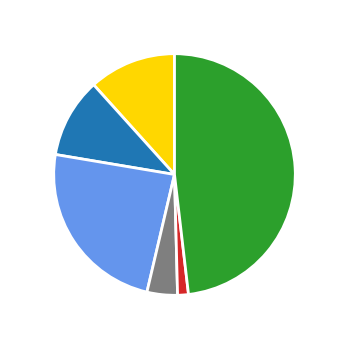
\includegraphics[width=\linewidth]{images/gw_sims/1n4_pie.png}
\end{minipage}
%
\begin{minipage}[t]{0.37\textwidth}\vspace{0pt}
\begin{tabular}{lrr}
\multicolumn{3}{c}{\textbf{Simulation results}} \\
\midrule
%% PASTE BELOW \/\/
\textcolor{Green}{Observed} & 532 & 48.1\% \\
\textcolor{Red}{Not observed} & 16 & 1.4\% \\
\textcolor{darkgray}{Not selected} & 45 & 4.1\% \\
\textcolor{NavyBlue}{Below dec limit} & 265 & 24.0\% \\
\textcolor{Blue}{Bad event time} & 118 & 10.7\% \\
\textcolor{BurntOrange}{Too close to Sun} & 129 & 11.7\% \\
\midrule
Visible events & 593 &  53.7\% \\
%% PASTE ABOVE /\/\
\end{tabular}
\end{minipage}
%
\begin{minipage}[t]{0.35\textwidth}\vspace{0pt}
\begin{tabular}{lr}
\multicolumn{2}{c}{\textbf{System: 1N4}} \\
\midrule
%% PASTE BELOW \/\/
Observing efficiency & 89.7\% \\
\midrule
Mean delay after     & \multirow{2}{*}{9.96 h} \\
event time           & \\
Mean delay after     & \multirow{2}{*}{1.58 h} \\
becoming visible     & \\
\midrule
Mean airmass         & 1.64 \\
%% PASTE ABOVE /\/\
\end{tabular}
\vfill
\end{minipage}

\end{center}
\caption[GW simulation results: 1N4 system]{Simulation results for a 1N4 system. This is the prototype system with 4 unit telescopes on a single mount currently deployed on La Palma.
}
\label{fig:gw_sim_1n4}
\end{figure}

% ---------

\begin{figure}[p]
    \begin{center}

    \begin{minipage}[t]{0.2\textwidth}\vspace{10pt}
    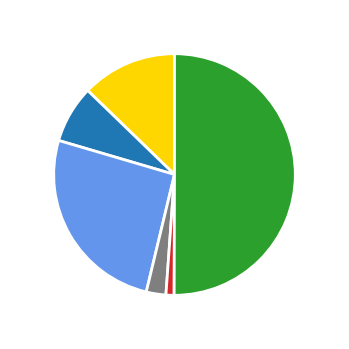
\includegraphics[width=\linewidth]{images/gw_sims/1n8_pie.png}
    \end{minipage}
    %
    \begin{minipage}[t]{0.37\textwidth}\vspace{0pt}
    \begin{tabular}{lrr}
    \multicolumn{3}{c}{\textbf{Simulation results}} \\
    \midrule
    %% PASTE BELOW \/\/
    \textcolor{Green}{Observed} & 553 & 50.0\% \\
    \textcolor{Red}{Not observed} & 12 & 1.1\% \\
    \textcolor{darkgray}{Not selected} & 29 & 2.6\% \\
    \textcolor{NavyBlue}{Below dec limit} & 285 & 25.8\% \\
    \textcolor{Blue}{Bad event time} & 85 & 7.7\% \\
    \textcolor{BurntOrange}{Too close to Sun} & 141 & 12.8\% \\
    \midrule
    Visible events & 594 &  53.8\% \\
    %% PASTE ABOVE /\/\
    \end{tabular}
    \end{minipage}
    %
    \begin{minipage}[t]{0.35\textwidth}\vspace{0pt}
    \begin{tabular}{lr}
    \multicolumn{2}{c}{\textbf{System: 1N8}} \\
    \midrule
    %% PASTE BELOW \/\/
    Observing efficiency & 93.1\% \\
    \midrule
    Mean delay after     & \multirow{2}{*}{10.06 h} \\
    event time           & \\
    Mean delay after     & \multirow{2}{*}{1.60 h} \\
    becoming visible     & \\
    \midrule
    Mean airmass         & 1.66 \\
    %% PASTE ABOVE /\/\
    & \\
    \end{tabular}
    \vfill
    \end{minipage}

    \end{center}
    \caption[GW simulation results: 1N8 system]{
        Simulation results for a 1N8 system. Note the distribution of events changes due to the different grid used, and the biggest gain in events observed is from the decreased number with sources not included in the selected tiles.
    }\label{fig:gw_sim_1n8}
\end{figure}

% ---------

\begin{figure}[p]
    \begin{center}

    \begin{minipage}[t]{0.2\textwidth}\vspace{10pt}
    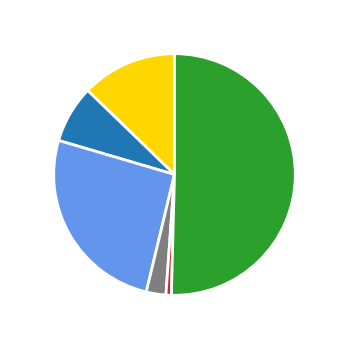
\includegraphics[width=\linewidth]{images/gw_sims/2n8_pie.png}
    \end{minipage}
    %
    \begin{minipage}[t]{0.37\textwidth}\vspace{0pt}
    \begin{tabular}{lrr}
    \multicolumn{3}{c}{\textbf{Simulation results}} \\
    \midrule
    %% PASTE BELOW \/\/
    \textcolor{Green}{Observed} & 557 & 50.4\% \\
    \textcolor{Red}{Not observed} & 8 & 0.7\% \\
    \textcolor{darkgray}{Not selected} & 29 & 2.6\% \\
    \textcolor{NavyBlue}{Below dec limit} & 285 & 25.8\% \\
    \textcolor{Blue}{Bad event time} & 85 & 7.7\% \\
    \textcolor{BurntOrange}{Too close to Sun} & 141 & 12.8\% \\
    \midrule
    Visible events & 594 &  53.8\% \\
    %% PASTE ABOVE /\/\
    \end{tabular}
    \end{minipage}
    %
    \begin{minipage}[t]{0.35\textwidth}\vspace{0pt}
    \begin{tabular}{lr}
    \multicolumn{2}{c}{\textbf{System: 2N8}} \\
    \midrule
    %% PASTE BELOW \/\/
    Observing efficiency & 93.8\% \\
    \midrule
    Mean delay after     & \multirow{2}{*}{9.89 h} \\
    event time           & \\
    Mean delay after     & \multirow{2}{*}{1.53 h} \\
    becoming visible     & \\
    \midrule
    Mean airmass         & 1.67 \\
    %% PASTE ABOVE /\/\
    & \\
    \end{tabular}
    \vfill
    \end{minipage}

    \end{center}
    \caption[GW simulation results: 2N8 system]{
        Simulation results for a 2N8 system. The improvements over the 1N8 system are a small gain in efficiency and decrease in mean delay time.
    }\label{fig:gw_sim_2n8}
\end{figure}

% ---------

\begin{figure}[p]
    \begin{center}

    \begin{minipage}[t]{0.2\textwidth}\vspace{10pt}
    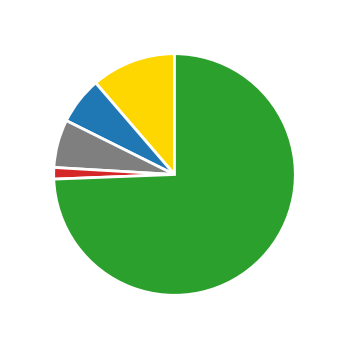
\includegraphics[width=\linewidth]{images/gw_sims/2n8&1s4_pie.png}
    \end{minipage}
    %
    \begin{minipage}[t]{0.37\textwidth}\vspace{0pt}
    \begin{tabular}{lrr}
    \multicolumn{3}{c}{\textbf{Simulation results}} \\
    \midrule
    %% PASTE BELOW \/\/
    \textcolor{Green}{Observed} & 822 & 74.4\% \\
    \textcolor{Red}{Not observed} & 17 & 1.5\% \\
    \textcolor{darkgray}{Not selected} & 71 & 6.4\% \\
    \textcolor{NavyBlue}{Below dec limit} & 0 & 0.0\% \\
    \textcolor{Blue}{Bad event time} & 70 & 6.3\% \\
    \textcolor{BurntOrange}{Too close to Sun} & 125 & 11.3\% \\
    \midrule
    Visible events & 910 &  82.4\% \\
    %% PASTE ABOVE /\/\
    \end{tabular}
    \end{minipage}
    %
    \begin{minipage}[t]{0.35\textwidth}\vspace{0pt}
    \begin{tabular}{lr}
    \multicolumn{2}{c}{\textbf{System: 2N8\+1S4}} \\
    \midrule
    %% PASTE BELOW \/\/
    Observing efficiency & 90.3\% \\
    \midrule
    Mean delay after     & \multirow{2}{*}{8.16 h} \\
    event time           & \\
    Mean delay after     & \multirow{2}{*}{1.66 h} \\
    becoming visible     & \\
    \midrule
    Mean airmass         & 1.63 \\
    %% PASTE ABOVE /\/\
    & \\
    \end{tabular}
    \vfill
    \end{minipage}

    \end{center}
    \caption[GW simulation results: 2N8+1S4 system]{
        Simulation results for a 2N8+1S4 system. Note as these sites use different grids they were simulated independently and the results combined.
    }\label{fig:gw_sim_2n8+1s4}
\end{figure}

% ---------

\begin{figure}[p]
    \begin{center}

    \begin{minipage}[t]{0.2\textwidth}\vspace{10pt}
    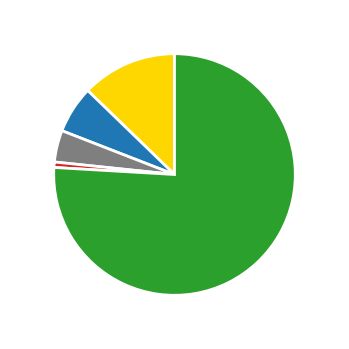
\includegraphics[width=\linewidth]{images/gw_sims/2n8+2s8_pie.png}
    \end{minipage}
    %
    \begin{minipage}[t]{0.37\textwidth}\vspace{0pt}
    \begin{tabular}{lrr}
    \multicolumn{3}{c}{\textbf{Simulation results}} \\
    \midrule
    %% PASTE BELOW \/\/
    \textcolor{Green}{Observed} & 839 & 75.9\% \\
    \textcolor{Red}{Not observed} & 8 & 0.7\% \\
    \textcolor{darkgray}{Not selected} & 47 & 4.3\% \\
    \textcolor{NavyBlue}{Below dec limit} & 0 & 0.0\% \\
    \textcolor{Blue}{Bad event time} & 70 & 6.3\% \\
    \textcolor{BurntOrange}{Too close to Sun} & 141 & 12.8\% \\
    \midrule
    Visible events & 894 &  80.9\% \\
    %% PASTE ABOVE /\/\
    \end{tabular}
    \end{minipage}
    %
    \begin{minipage}[t]{0.35\textwidth}\vspace{0pt}
    \begin{tabular}{lr}
    \multicolumn{2}{c}{\textbf{System: 2N8+2S8}} \\
    \midrule
    %% PASTE BELOW \/\/
    Observing efficiency & 93.8\% \\
    \midrule
    Mean delay after     & \multirow{2}{*}{7.69 h} \\
    event time           & \\
    Mean delay after     & \multirow{2}{*}{1.57 h} \\
    becoming visible     & \\
    \midrule
    Mean airmass         & 1.64 \\
    %% PASTE ABOVE /\/\
    & \\
    \end{tabular}
    \vfill
    \end{minipage}

    \end{center}
    \caption[GW simulation results: 2N8+2S8 system]{
        Simulation results for a 2N8+2S8 system. The largest gain over the northern hemisphere-only system is the removal of the declination limited events, meaning more event sources are visible. The efficiency remains the same but there is a notable improvement in the post-event delay times.
    }\label{fig:gw_sim_2n8+2s8}
\end{figure}

% ---------

\begin{figure}[p]
    \begin{center}

    \begin{minipage}[t]{0.2\textwidth}\vspace{10pt}
    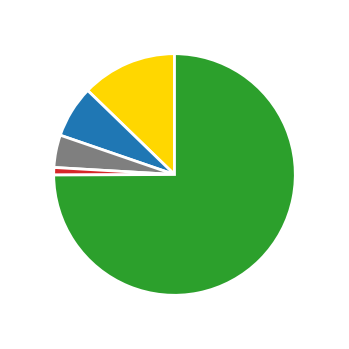
\includegraphics[width=\linewidth]{images/gw_sims/2n8+2k8_pie.png}
    \end{minipage}
    %
    \begin{minipage}[t]{0.37\textwidth}\vspace{0pt}
    \begin{tabular}{lrr}
    \multicolumn{3}{c}{\textbf{Simulation results}} \\
    \midrule
    %% PASTE BELOW \/\/
    \textcolor{Green}{Observed} & 828 & 74.9\% \\
    \textcolor{Red}{Not observed} & 11 & 1.0\% \\
    \textcolor{darkgray}{Not selected} & 48 & 4.3\% \\
    \textcolor{NavyBlue}{Below dec limit} & 0 & 0.0\% \\
    \textcolor{Blue}{Bad event time} & 77 & 7.0\% \\
    \textcolor{BurntOrange}{Too close to Sun} & 141 & 12.8\% \\
    \midrule
    Visible events & 887 &  80.3\% \\
    %% PASTE ABOVE /\/\
    \end{tabular}
    \end{minipage}
    %
    \begin{minipage}[t]{0.35\textwidth}\vspace{0pt}
    \begin{tabular}{lr}
    \multicolumn{2}{c}{\textbf{System: 2N8+2K8}} \\
    \midrule
    %% PASTE BELOW \/\/
    Observing efficiency & 93.3\% \\
    \midrule
    Mean delay after     & \multirow{2}{*}{7.69 h} \\
    event time           & \\
    Mean delay after     & \multirow{2}{*}{1.55 h} \\
    becoming visible     & \\
    \midrule
    Mean airmass         & 1.64 \\
    %% PASTE ABOVE /\/\
    & \\
    \end{tabular}
    \vfill
    \end{minipage}

    \end{center}
    \caption[GW simulation results: 2N8+2K8 system]{
        Simulation results for a 2N8+2K8 system. Note it makes very little difference to the results if the southern site is at Siding Spring or Mt Kent, compared to the huge gain from either compared to just La Palma.
    }\label{fig:gw_sim_2n8+2k8}
\end{figure}

% ---------

\clearpage

\begin{table}[t]
    \begin{center}
    \begin{tabular}{c|cccc|c|cc|c} % chktex 44

    \multirow{2}{*}{System} &
    \multicolumn{4}{c|}{Observed within \ldots} &
    Observing &
    \multicolumn{2}{c|}{Mean delay time \ldots} &
    Mean
    \\
    &
    1h &
    6h &
    12h &
    24h &
    efficiency&
    event &
    visible &
    airmass
    \\
    \midrule
    1N4 & 5.9\% & 16.5\% & 26.2\% & 48.1\% & 89.7\% & 9.96 h & 1.58 h & 1.64 \\
    1N8 & 6.8\% & 16.9\% & 27.1\% & 50.0\% & 93.1\% & 10.06 h & 1.60 h & 1.66 \\
    2N8 & 7.2\% & 17.3\% & 27.9\% & 50.4\% & 93.8\% & 9.89 h & 1.53 h & 1.67 \\
    &&&&&&&&\\
    1S4 & 8.8\% & 18.8\% & 27.9\% & 47.1\% & 87.7\% & 9.39 h & 1.64 h & 1.61 \\
    1S8 & 10.3\% & 20.6\% & 31.1\% & 49.2\% & 91.0\% & 8.81 h & 1.52 h & 1.63 \\
    2S8 & 11.1\% & 21.2\% & 31.8\% & 49.9\% & 92.1\% & 8.67 h & 1.47 h & 1.64 \\
    &&&&&&&&\\
    2K8 & 10.8\% & 20.9\% & 31.3\% & 50.9\% & 92.3\% & 9.02 h & 1.46 h & 1.65 \\
    &&&&&&&&\\
    1N8+1S8 & 17.1\% & 36.8\% & 52.5\% & 74.8\% & 92.5\% & 7.82 h & 1.63 h & 1.63 \\
    2N8+1S8 & 17.6\% & 37.2\% & 52.9\% & 75.2\% & 93.0\% & 7.75 h & 1.59 h & 1.64 \\
    2N8+2S8 & 18.4\% & 37.7\% & 53.8\% & 75.9\% & 93.8\% & 7.69 h & 1.57 h & 1.64 \\
    &&&&&&&&\\
    2N8+2K8 & 18.2\% & 38.0\% & 52.8\% & 74.9\% & 93.3\% & 7.69 h & 1.55 h & 1.64 \\
    &&&&&&&&\\
    2N8+1S4* & 16.0\% & 35.7\% & 50.3\% & 74.4\% & 90.3\% & 8.16 h & 1.66 h & 1.63 \\
    2N8+1S8* & 17.6\% & 37.2\% & 53.0\% & 75.2\% & 93.0\% & 7.76 h & 1.60 h & 1.64 \\
    2N8+2S8* & 18.4\% & 37.7\% & 53.7\% & 75.9\% & 93.8\% & 7.70 h & 1.58 h & 1.64 \\

    \end{tabular}
    \end{center}
    \caption[GW simulation results summary table]{
        Summary of simulation results. Systems marked with an asterisk (*) were not simulated together, but were instead combined from the individual simulations for each site.
    }\label{tab:gw_sim_results}
    \end{table}

\end{colsection}

% ~~~~~~~~~~~~~~~~~~~~

\subsection{Analysis of simulation results}
\label{sec:gw_sim_analysis}
\begin{colsection}

The results of the gravitational wave follow-up simulations support two conclusions: the addition of the southern site provides a huge benefit to the number of sources that can be observed, while adding further telescopes at a single site provides a much more modest benefit. \aref{fig:gw_sim_results} summarises the simulated post-event delay times for different expected stages of \gls{goto} deployment.

\begin{figure}[t]
    \begin{center}
        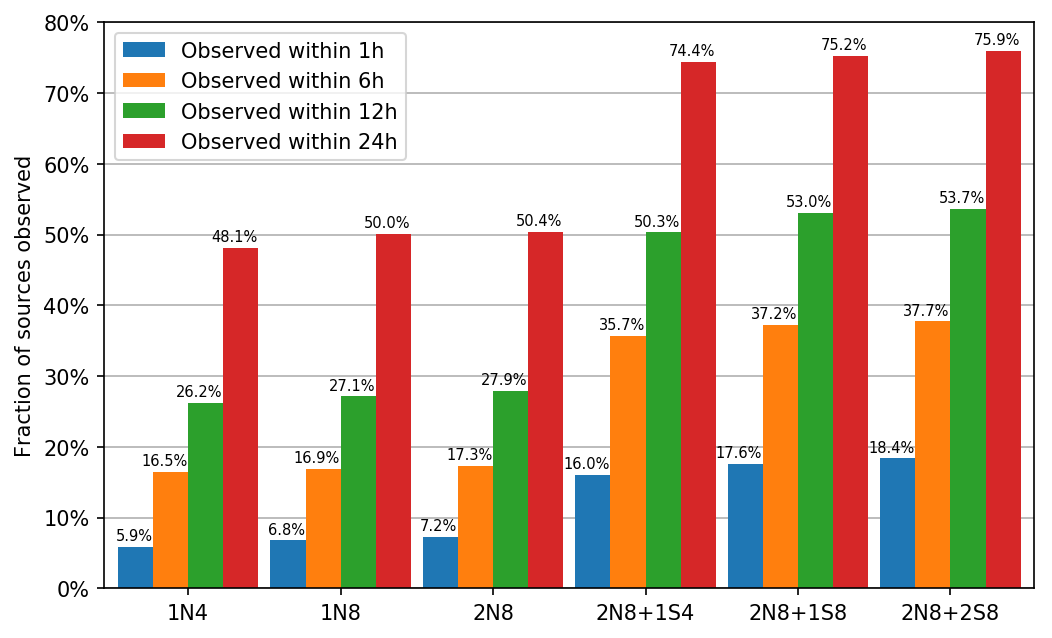
\includegraphics[width=\linewidth]{images/gw_sims/results.png}
    \end{center}
    \caption[Simulation delay time for different GOTO systems]{
        Post-event delay in observing gravitational wave event sources for six deployment stages of the GOTO system.
    }\label{fig:gw_sim_results}
\end{figure}

The reason for the first conclusion is obvious: adding a site in the southern hemisphere opens up a large number of sources that are physically incapable of being observed from La Palma. The second comes about essentially because the efficiency of a single GOTO system is already very high. \aref{fig:gw_sim_1n8} shows the 1N8 system already observes 93.1\% of all sources visible from La Palma, and a majority of those not observed were outside of the selected tiles (29 events) compared to just not being observed (12 events). The addition of the second GOTO-8 system as shown in \aref{fig:gw_sim_2n8} moves just 4 events from ``not observed'' to ``observed'', and can't make any changes to any of the other categories. The delay time does decrease, but again only be a small amount.

The above conclusions are perhaps most visible by comparing the results in \aref{tab:gw_sim_results} for the 2N8 system to the 1N8+1S8 system, where there is a clear gain in the number of sources observed within the 24 hours (50.4\% to 74.8\%). Therefore, on these metrics alone, it would be far better to prioritise deploying a second mount in Australia before adding another on La Palma. There are numerous practical reasons why this is not the priority of the collaboration, and \aref{sec:survey_sims} below illustrates that multiple telescopes at a single site are much more important to the all-sky survey cadence.

Regarding the choice of southern site, there is very little difference between results from Siding Spring and from Mt Kent. Comparing the 2S8 and 2K8 simulation results in \aref{tab:gw_sim_results} show Mt Kent has a small advantage in terms of number of events observed, but Siding Spring has a lower mean delay time. Overall the difference was deemed small enough to negate the difference between the two sites, and in most cases the ``S'' simulations are considered as representative of either site.

Another factor to emerge from these simulations is the difference between two independent systems in either hemisphere vs one combined system that uses a common database. This emerged as important as it was desired to simulate the 2N8+1S4 system, as a plausible future stage of GOTO's deployment while the southern site is being commissioned similar to the current situation on La Palma. As mentioned previously the simulations require all telescopes to be observing using the same grid, as otherwise it is impossible at this time to map the common tiles between them. However it is possible to consider the two cases, 2N8 and 1S4, separately as independent simulations and then combine the results. For the event counts the logic is fairly straightforward: if an event is observed by either site it counts as being observed. To get the delay times it was necessary to consider which site observed it first, and then use the delay times and airmass of that observation. Using this method the results shown in \aref{fig:gw_sim_2n8+1s4} were derived. The same method could also be used in situations where the two sites could be simulated together. For example comparing the 2N8+2S8 simulation to the combined result of the 2N8 and 2S8 simulations, given as 2N8+2S8* in \aref{tab:gw_sim_results}. The exact same events fell into the same categories as shown in \aref{fig:gw_sim_2n8+2s8}, and the only difference is a small hit to the delay time when the sites are not simulated together. This is due to some individual cases where the difference can be quite pronounced. For large skymaps with lots of tiles within the shared area of the sky visible form both sites (roughly $\pm$\SI{30}{\degree}) one site can complete observations of this region even if it can't see the source, meaning once the other telescope opens and starts observing a large area of the skymap that doesn't contain the source has already been excluded. This is only the case when both sites are observing using a shared database, as the second site needs to know what the first site has already observed.

\end{colsection}

% ~~~~~~~~~~~~~~~~~~~~

\end{colsection}

% ########################################

\newpage
\section{All-sky survey simulations}
\label{sec:survey_sims}
\begin{colsection}

% ~~~~~~~~~~~~~~~~~~~~

\begin{colsection}

Almost as critical to the \gls{goto} project as the gravitational wave follow-up operations is carrying out the all-sky survey. Therefore in parallel to the gravitational wave simulations further simulations were carried out in order to quantify what benefit additional telescopes and sites will have on the survey. It was also an opportunity to consider different survey methods before implementing them in the real scheduling system. Unlike the gravitational wave simulations it is also possible to compare the simulated results for a single GOTO-4 system on La Palma to the actual observations the live system has taken over its first 5 months operating.

\end{colsection}

% ~~~~~~~~~~~~~~~~~~~~

\subsection{Simulating survey observations}
\label{sec:survey_sim_methods}
\begin{colsection}

Simulating the all-sky survey is more straightforward than the gravitational wave simulations, as there isn't the added complication of processing the \gls{lvc} skymap or checking the visibility of the source coordinates. Instead the only set up that is needed is to fill the observing database with the all-sky survey Mpointings and run the fake pilot calling the usual scheduler commands.

The only drawback to this method is the time taken. Unlike the gravitational wave simulations the simulation can't be finished early if the source is not visible, or stopped once the source has been observed. Instead the fake pilot needs to simulate the full 24 hours of observations, for however many days the simulation is run for. The same simplifications detailed in \aref{sec:multi_site} still apply, so each loop still skips approximately 4 minutes of simulation time until the observation has completed. A full simulation of a year of observations including both sites (therefore observing for approximately to 20 hours each day) requires 1.1 million steps, and with each simulation loop taking approximately 2 seconds (the scheduler check takes the majority of the time) the full simulation takes approximately 60 hours. This compares to at most 16 hours for the multi-site gravitational wave simulations.

Due to the full simulations requiring a large time investment only a few of these were carried out. Instead, a simplified version of the simulation code was developed that could produce the same results much faster. This `lite' script did away with the scheduler and database code, and instead at each step just finds the highest altitude tiles that have been observed the least times and takes them as the return pointings from the scheduler. This is a massive simplification of the scheduling functions, however the result is effectively the same and the same simulations are 15--20 times faster to run. Therefore a majority of the simulations discussed in this section use this much faster `lite' script. The other benefit of this method was making it much easier to modify the ``scheduling'' function to test different methods, as discussed in \aref{sec:survey_sim_meridian}, without yet needing the rewrite the actual \gls{gtecs} scheduler.

\end{colsection}

% ~~~~~~~~~~~~~~~~~~~~

\subsection{Multi-telescope simulation results}
\label{sec:survey_sim_results}
\begin{colsection}

Simulations were carried out for different combinations of \gls{goto} telescopes and sites, similar to the gravitational wave response simulations detailed in \aref{sec:gw_sims}. Simulations were run for 365 days starting semi-arbitrarily on the 21st of February 2019, which was the date the current ongoing survey started on La Palma.

Fewer simulations were carried out when compared to the gravitational wave simulations. This is partially due to them taking longer to run, but also as unlike the GW simulations there is no practical way or reason to combine the results from different sites. It is also not possible to combine the results of telescopes observing on different grids: unlike the GW simulations, where the grid was the means to observe the event source location, for these simulations the grid is the target being observed and the results are directly tied to the grid used.

The results of each simulation are given in \aref{tab:survey_sim_results}. \aref{fig:survey_sim_1n4} shows the final tile coverage map for the 1N4 system, in which each tile in the GOTO-4 grid is coloured by the number of times it was observed. \aref{fig:survey_sim_2n8+2s8} gives the same for the final 2N8+2S8 system.

% ---------

\begin{figure}[p]
    \begin{center}
        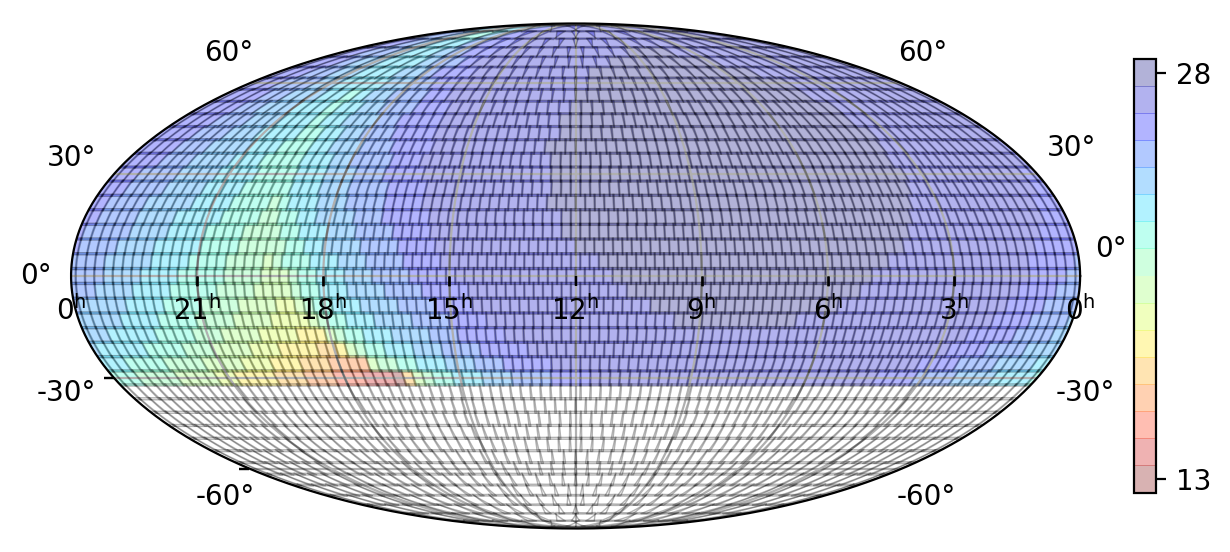
\includegraphics[height=190pt]{images/survey_sims/365_1N4_lite.png}
    \end{center}
    \caption[All-sky survey simulation results: 1N4 system]{
        All-sky survey simulation coverage map for a 1N4 system, as currently deployed on La Palma. Tiles are coloured by the number of times they were observed over the 365 simulated nights. Tiles in white are those not visible from the northern site.
    }\label{fig:survey_sim_1n4}
\end{figure}

\begin{figure}[p]
    \begin{center}
        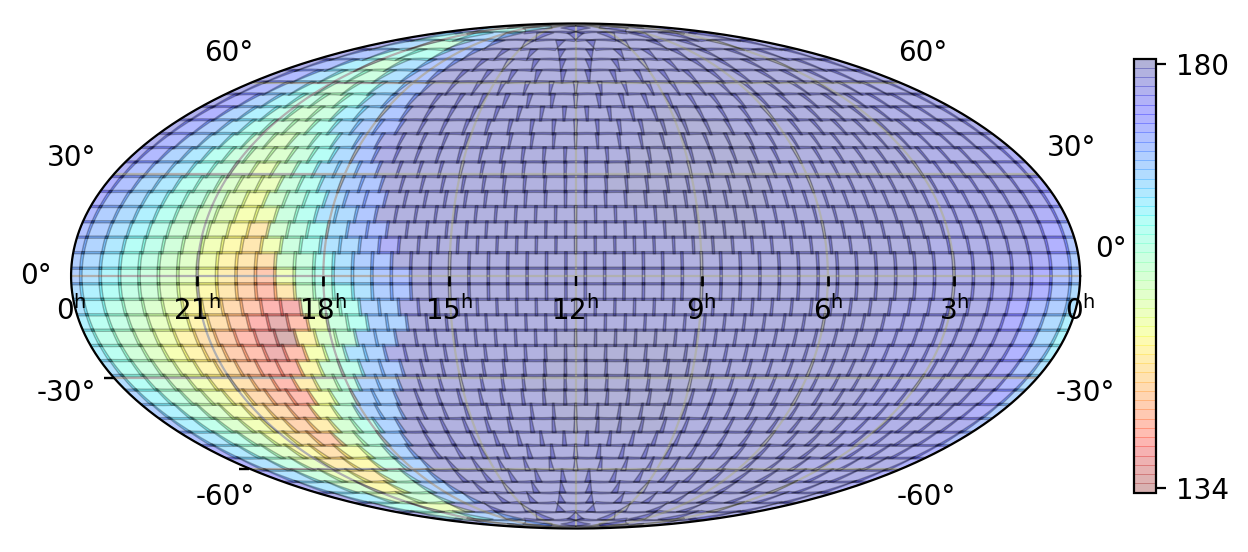
\includegraphics[height=190pt]{images/survey_sims/365_2N8+2S8_lite.png}
    \end{center}
    \caption[All-sky survey simulation results: 2N8+2S8 system]{
        All-sky survey simulation coverage map for a 2N8+2S8 system, the ultimate design goal of the \gls{goto} collaboration. Note the colour scale has changed from \aref{fig:survey_sim_1n4}, the grid has changed to the GOTO-8 tiles and the region which was previously not visible from just the north has been filled in.
    }\label{fig:survey_sim_2n8+2s8}
\end{figure}

% ---------

\clearpage

\begin{table}[t]
    \begin{center}
    \begin{tabular}{c|cc|c|c|c} % chktex 44

    \multirow{2}{*}{System} &
    \multicolumn{2}{c|}{Fraction of sky observed} &
    No.\ times &
    Mean cadence &
    Mean observed
    \\
    &
    each night &
    over 1y &
    tiles observed &
    (days) &
    airmass
    \\
    \midrule
    1N4* & 4.3\%--6.5\% & 76.5\% & 26 (13--28) & $10.0\pm1.8$ & $1.6\pm0.4$ \\
    &&&&&\\
    1N4 & 4.3\%--6.4\% & 76.5\% & 26 (13--28) & $10.1\pm1.8$ & $1.6\pm0.3$ \\
    1N8 & 9.5\%--14.0\% & 74.2\% & 58 (34--62) & $4.6\pm0.7$ & $1.6\pm0.4$ \\
    2N8 & 19.0\%--28.1\% & 74.2\% & 117 (68--123) & $2.3\pm0.4$ & $1.6\pm0.4$ \\
    &&&&&\\
    1N8+1S8 & 23.2\%--24.1\% & 99.9\% & 87 (67--91) & $3.4\pm0.3$ & $1.5\pm0.4$ \\
    2N8+1S8 & 33.0\%--37.3\% & 99.9\% & 130 (98--138) & $2.3\pm0.2$ & $1.6\pm0.4$ \\
    2N8+2S8 & 46.3\%--48.1\% & 99.9\% & 173 (134--180) & $1.7\pm0.1$ & $1.5\pm0.4$ \\
    &&&&&\\
    2N8+2K8 & 46.8\%--48.3\% & 99.8\% & 174 (134--181) & $1.7\pm0.1$ & $1.6\pm0.4$ \\

    \end{tabular}
    \end{center}
    \caption[All-sky survey simulation results summary table]{
        Summary of all-sky survey simulation results. The first 1N4 simulation, marked with an asterisk (*), was the only one carried out using the full scheduler and database system. All the other simulations used the `lite' script. The fraction of the sky observed each night is given as a range over the course of a year, and the number of times each tile was observed gives the mean of all tiles as well as the the minimum and maximum.
    }\label{tab:survey_sim_results}
\end{table}

\end{colsection}

% ~~~~~~~~~~~~~~~~~~~~

\subsection{Analysis of simulation results}
\label{sec:survey_sim_analysis}
\begin{colsection}

The results of the all-sky survey simulations show, as expected, that the greatest benefit to the survey cadence comes from increasing the number of telescopes at each site. \aref{fig:survey_sim_results} plots the change in mean cadence and fraction of the sky observed each night for different expected stages of \gls{goto} deployment.

\begin{figure}[t]
    \begin{center}
        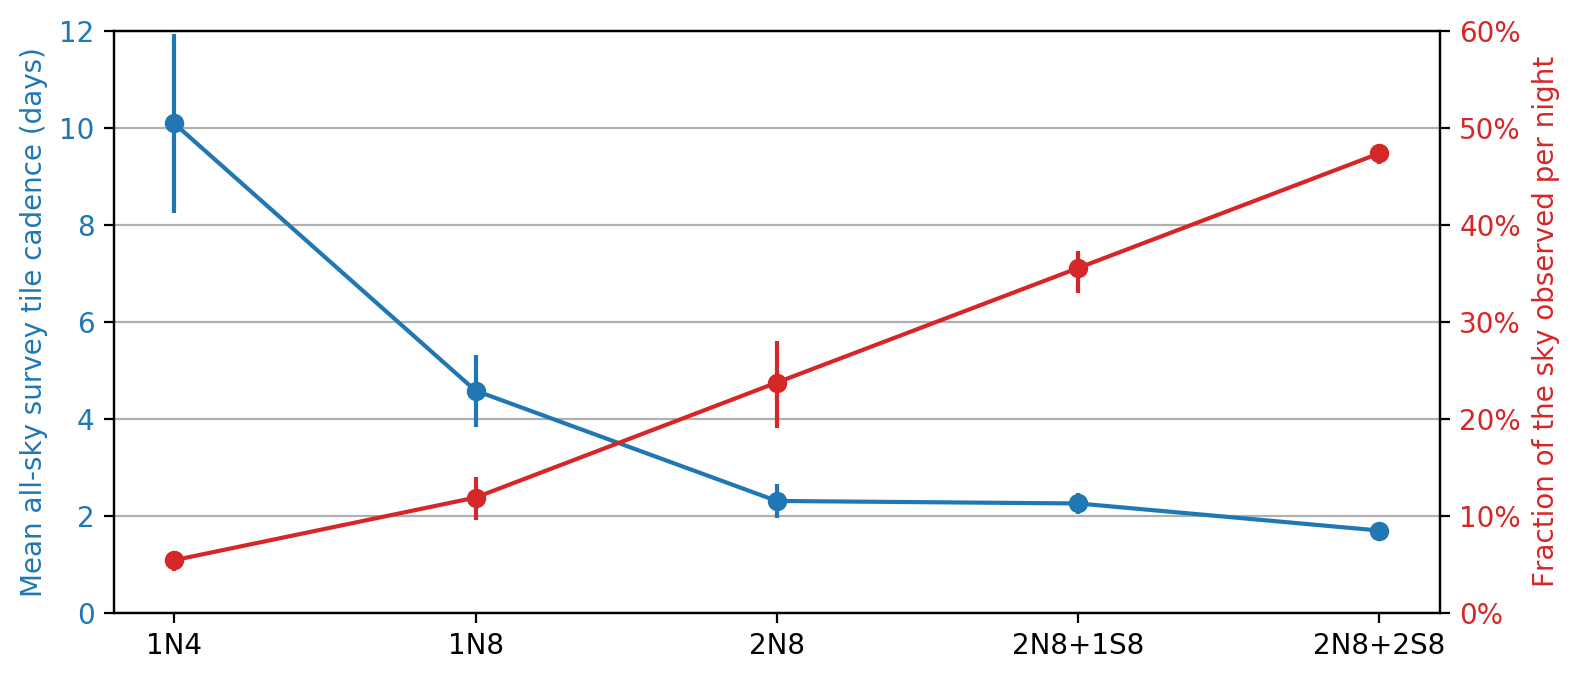
\includegraphics[width=\linewidth]{images/survey_sims/results.png}
    \end{center}
    \caption[Tile cadence and nightly sky observation for different GOTO systems]{
        Mean tile cadence and fraction of the sky observed each night for five deployment stages of the GOTO system. Error bars on the cadence show the standard deviation for all the tiles observed across the sky, while error bars on the observed fraction show the minimum and maximum nightly observed fraction arising from differing night lengths throughout the year.
    }\label{fig:survey_sim_results}
\end{figure}

The improvement in tile observation cadence roughly follows the expected trend that doubling the instantaneous field of view would double the number of observations carried out in one night and therefore halve the time between observations. With the current GOTO-4 system (1N4) the simulations predict approximately 10 days between tile observations, reduced to approximately 5 days with the upgrade to the full GOTO-8 system (1N8) and then halving again to 2.5 days with the addition of the second GOTO-8 telescope (2N8). Adding a single GOTO-8 telescope in Australia will leave the tile cadence effectively unchanged, which is simply a matter of geometry. Adding a site in Australia increases the total amount of the sky that is visible over the year from roughly 75\% to practically 100\% (from La Palma the single tile over the north pole is not visible, as discussed in \aref{sec:algorithms}), an increase of one third in the area needed to cover. Adding just one GOTO-8 telescope in the south corresponds to a one third increase in the amount of sky that can be observed during the year, and therefore the efficiency (and cadence) remains the same. Adding the second telescope in Australia correspondingly decreases the further, although as this is only increasing the overall instantaneous field of view by one third the cadence is only reduced by a third from 2.5 to 1.66 days.

The increase of the fraction of the sky observed each night is fairly linear, from both the increased instantaneous field of view and the opening of the lower declination sky with the southern site. The variation over the course of the year comes from seasonal variation in the length of then night, it increases as more telescopes are added in the north and is reduced to effectively nil with equal number of telescopes in both hemispheres.

Again including Mt Kent gives effectively the same results as using Siding Spring, which is why the `S' simulations were taken as representative of either southern site. The only slight notable difference is the reduction in the amount of sky visible over the whole year, as like La Palma Mt Kent can't see the single tile over the southern pole.

\end{colsection}

% ~~~~~~~~~~~~~~~~~~~~

\subsection{Comparison of simulations to real observations}
\label{sec:survey_sim_150}
\begin{colsection}

Unlike the gravitational wave simulations, the results of the survey simulations can be compared to the real observations carried out by the existing telescope on La Palma. The current phase of the \gls{goto} project began on the night of the 21st of February 2019. This was the first night observing fully robotically with the complete set of four unit telescopes, and marks the start of the ongoing all-sky survey. The first 5 months of observations spans exactly 150 days, from the night beginning on the 21st of February to the night ending on the 21st of July, and this provides the benchmark to compare with simulations over the same period.

All the all-sky survey simulations described in the previous section were started on the 21st of February. \aref{fig:150} shows the number of tiles observed each night by the real \gls{goto} on La Palma and the corresponding 1N4 simulation, restricted to the first 150 days. Over the entire period 16,146 on-grid observations were carried out by the telescope on La Palma, of which 85\% were survey pointings. In comparison the simulation produced 21,300 observations over the same period.

\begin{figure}[t]
    \begin{center}
        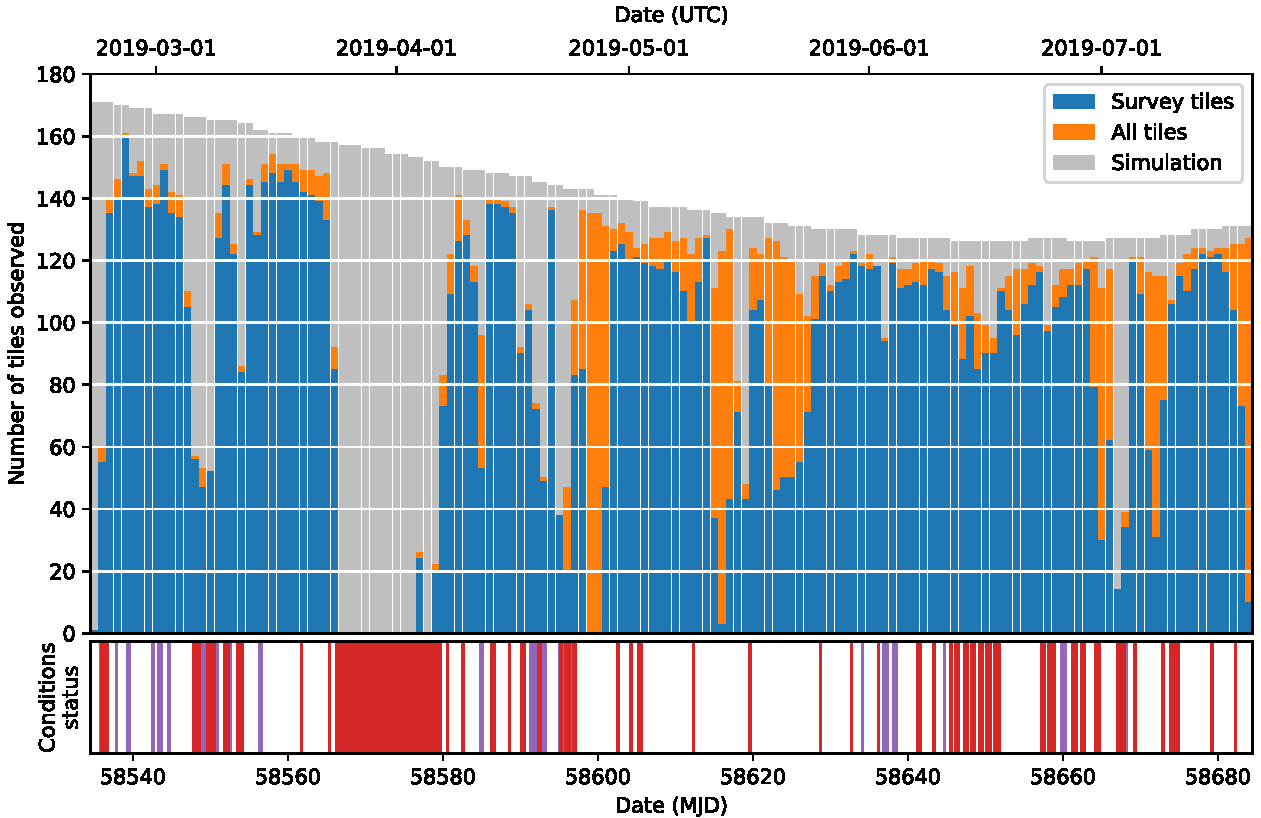
\includegraphics[width=\linewidth]{images/150.pdf}
    \end{center}

    \caption[Observations carried out in the first 150 days of the 4-UT all-sky survey]{
        Observations carried out in the first 150 days of the 4-UT all-sky survey. The count of survey observations is shown in the upper plot, with the number of survey tiles observed each night shown in \textcolor{Blue}{blue}, and any extra observations (of gravitational wave events, GRB triggers or manually-inserted pointings) shown in \textcolor{BurntOrange}{orange}. The background \textcolor{Gray}{grey} bars show the number of tiles observed on the same nights by the 1N4 survey simulation. The lower ``barcode'' plot shows the periods when the conditions flags were recorded as bad, either due to weather (\textcolor{Red}{red}) or hardware errors (\textcolor{Purple}{purple}).
    }\label{fig:150}
\end{figure}

The simulated observations can be considered the idealised case, and the real observations carried out differ from the target provided by the simulation in three ways:

\begin{itemize}
    \item Firstly the real system on La Palma is affected by periods of bad weather conditions, shown by the red and purple bars below the main plot. The conditions being bad stops observations and reduces the number carried out each night, notably there was one bad period of weather in late March and early April when the dome couldn't open for over a week. The simulations don't include any consideration of the weather factors, although the code exists to simulate periods of bad conditions and future simulations could include the real weather profile over the same period. On some nights there will also be other reasons for observations to be paused that weren't reflected in the conditions logs, for example switching to manual mode to carry out calibration tests or on-site work.

    \item Secondly the real system had to deal with multiple distractions from observing the all-sky survey. The orange bars show the non-survey observations, which take up a significant amount of time (15\% of all observations). Some nights are almost entirely orange, these correspond to LVC gravitational wave triggers with particularly large skymaps visible from La Palma such as S190425z and S190426c in late April, multiple events during May and S190720a just before the end of the period in mid-July. Other orange patches represent observations of smaller \gls{gw} skymaps, \gls{grb} triggers or other manually-inserted targets. These likewise are not considered in the simulations.

    \item Finally there is still a visible offset between the number of real observations taken in nights with clear conditions and the number predicted by the simulations. This discrepancy will be due to the values used within the simulation for camera readout and slew time not matching up precisely with the actual times, and future simulations will be able to be calibrated more accurately against real data.
\end{itemize}

\aref{fig:survey_real_150} shows the coverage map for the real observations in the first 150 days, while \aref{fig:survey_sim_1n4_150} shows the same for the 1N4 simulation. The physical sky coverage is very similar, the real observations cover 2,135 of the 2,913 GOTO-4 grid tiles at least once while the simulation covers 2,187. The reason for the discrepancy is that initially the real system used an altitude limit of \SI{35}{\degree} for the all-sky survey, which was lowered to \SI{30}{\degree} in May. This is visible in the bottom row of tiles in \aref{fig:survey_real_150}. The simulations all assume a constant \SI{30}{\degree} limit.

The major difference in the coverage between the real and simulated results is in the number of times each tile as observed. \aref{fig:survey_real_150} shows the most a single tile was observed was nine times, meaning the database was on the 9th pass over the visible sky at the end of the period. \aref{fig:survey_sim_1n4_150} shows the simulated results reach the 13th pass. This is entirely due to the combination of factors above meaning that all-sky simulations overestimate the number of observations taken during the 150 days. The mean tile cadence of the real observations is $14\pm4$, compared to $10\pm2$ from the simulation. It is clear that future simulations need to take into account time lost to weather and other observations in order to accurately predict the output of the real system. Overall though, aside from the constant offset visible in \aref{fig:150}, the simulations do seem to provide a reasonable approximation of what \gls{goto} could observe in this idealised case.

\begin{figure}[p]
    \begin{center}
        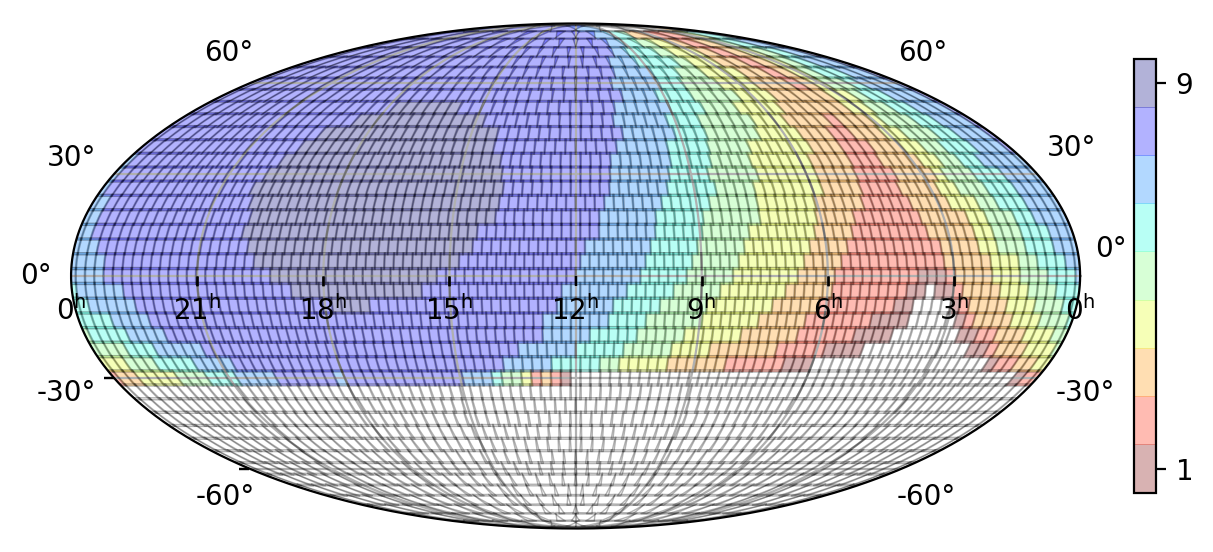
\includegraphics[height=190pt]{images/survey_sims/150_1N4_real.png}
    \end{center}

    \caption[Real survey observations over 150 days]{
        Real all-sky survey coverage map of observations over the first 150 days, from 21st February to 21st July. Tiles are coloured by the number of times they were observed during that period, and tiles in white were not observed.
    }\label{fig:survey_real_150}
\end{figure}

\begin{figure}[p]
    \begin{center}
        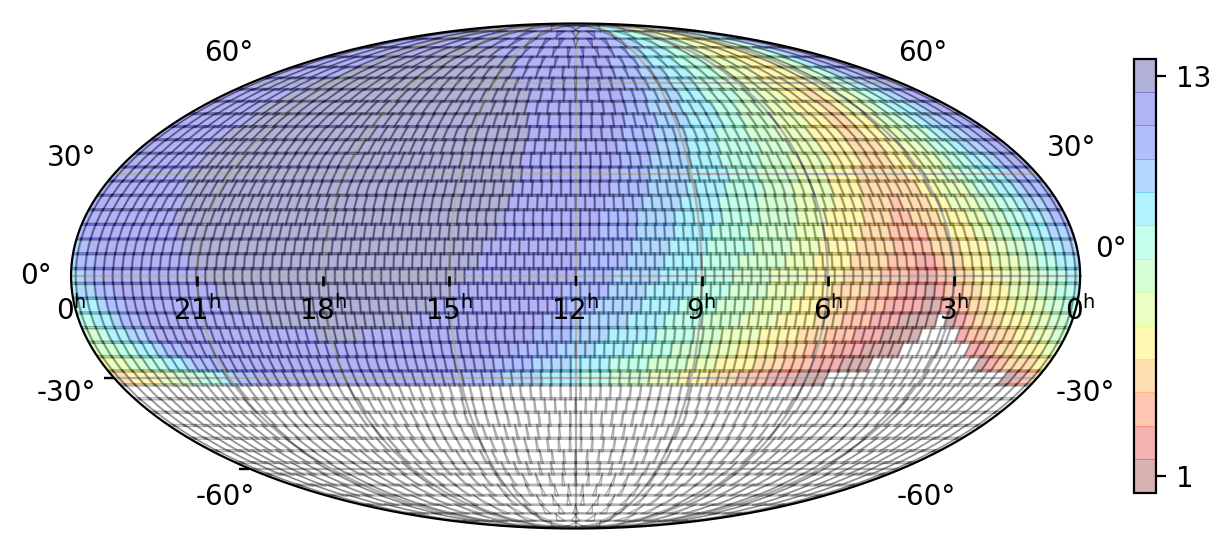
\includegraphics[height=190pt]{images/survey_sims/150_1N4_lite.png}
    \end{center}

    \caption[1N4 survey simulation observations over 150 days]{
        1N4 all-sky survey simulation coverage map over the first 150 days. Compare to \aref{fig:survey_sim_1n4} for the coverage over the entire 1-year simulation.
    }\label{fig:survey_sim_1n4_150}
\end{figure}

\clearpage

\end{colsection}

% ~~~~~~~~~~~~~~~~~~~~

\subsection{An alternative, meridian limited survey method}
\label{sec:survey_sim_meridian}
\begin{colsection}

One of the problems with the current scheduling system for the all-sky survey is that it leads to observations being carried out at low airmasses. Due to how the scheduler ranks tiles, discussed in \aref{sec:scheduler}, when all the visible survey tiles have been observed the same number of times then the scheduler will chose between them based on the airmass tiebreak parameter (unlike tiles linked to skymaps all survey tiles have equal weights, so the tiebreaking algorithm examined in \aref{sec:scheduler_sims} is simplified). This results in the scheduler always selecting tiles as soon as they rise if they have been observed fewer times than any others currently visible, and this means survey tiles are often observed at low airmasses leading to poor data quality. In practice images with poor data quality will be rejected by the analysis pipelines anyway, so arguably it is wasting the telescope's time to observe them.

One possible method to fix this problem and improve the data quality  is to implement an cut-off when observing survey tiles. This would not be a limit based on altitude or airmass, because that would exclude tiles close to the site declination limits (such as near the north pole from La Palma) which could never rise above the limit. Instead observations could be limited based on distance from the meridian, which in practice is limiting target's right ascension compared to the current \gls{lst}. By limiting to the current \gls{lst} $\pm$ a certain limit this is defining a strip surrounding the meridian within which survey tiles are valid and outside of which they are not.

In order to see the consequences of this method several simulations were carried out by modifying the all-sky survey `lite' script to limit based on the \gls{lst} at each step of the simulation. Each was run using the 1N4 system. The results of these simulations are given in \aref{tab:survey_sim_meridian}, for different meridian limits and the unlimited case for comparison. \aref{fig:survey_sim_airmass_365} shows the change in distribution of airmasses between the existing unlimited method and when restricting observations to a \SI{20}{\degree} wide strip ($\pm\SI{10}{\degree}$) at the meridian. \aref{fig:survey_sim_airmass_normal} shows the mean airmass each tile was observed in the first month using the existing method, while \aref{fig:survey_sim_airmass_meridian} shows the same using the limit.

\begin{figure}[p]
    \begin{center}
        \begin{minipage}[t]{0.49\textwidth}\vspace{10pt}
            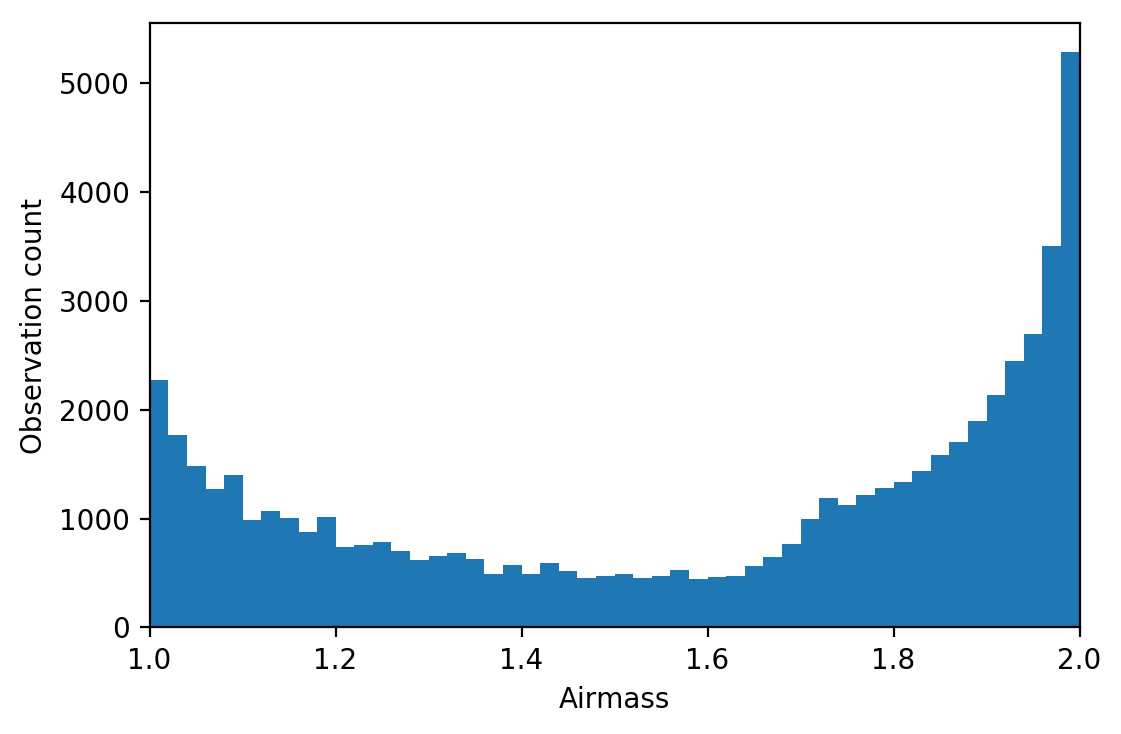
\includegraphics[height=140pt]{images/survey_sims/365_1N4_lite_airmass3.png}
        \end{minipage}
        \begin{minipage}[t]{0.49\textwidth}\vspace{10pt}
            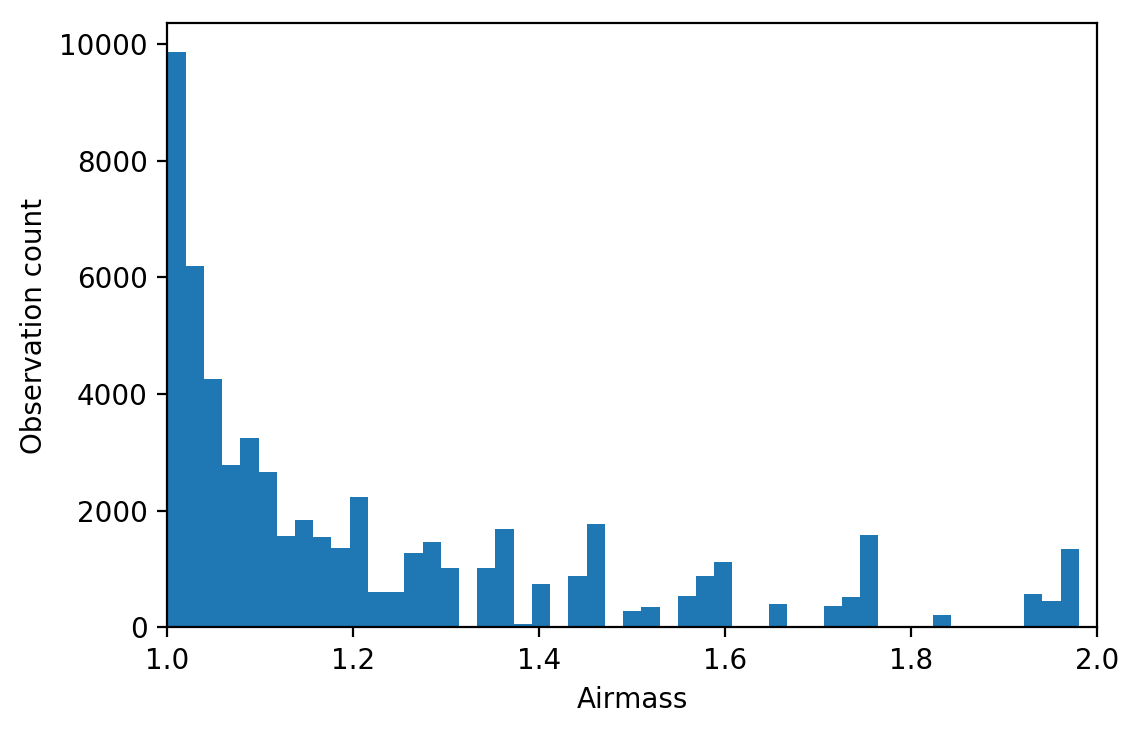
\includegraphics[height=140pt]{images/survey_sims/365_1N4_meridian_airmass3.png}
        \end{minipage}
    \end{center}

    \caption[Airmass distribution over a year of observations]{
        Airmass distribution over a year of observations with the 1N4 system, for the normal unlimited case (left) and the meridian $\pm\SI{10}{\degree}$ case (right).
    }\label{fig:survey_sim_airmass_365}
\end{figure}

\begin{figure}[p]
    \begin{center}
        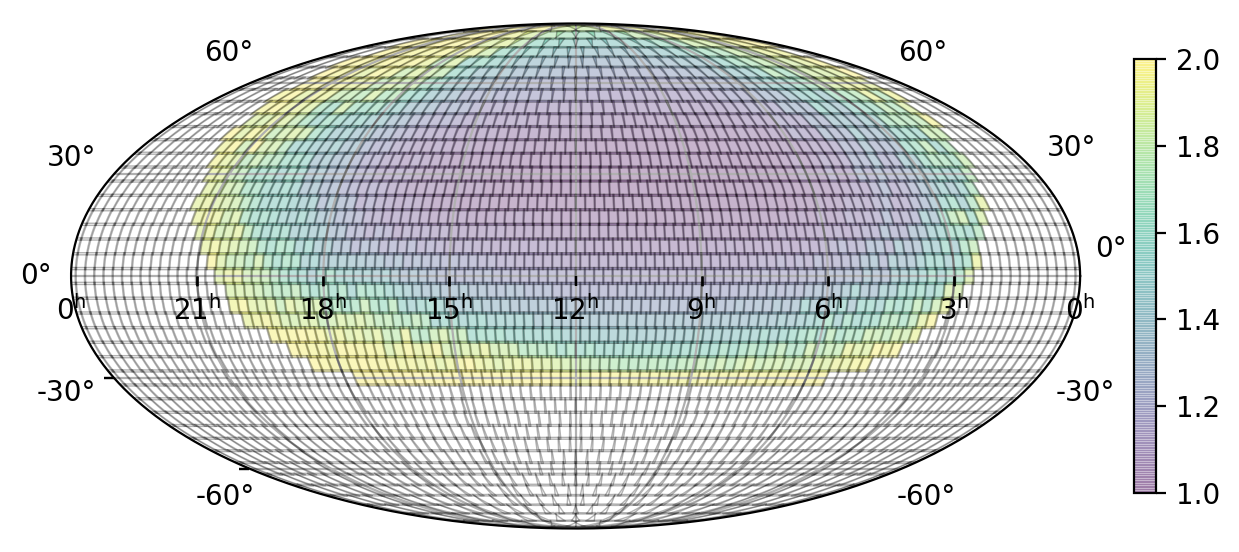
\includegraphics[width=0.7\linewidth]{images/survey_sims/30_1N4_lite_airmass.png}
    \end{center}

    \caption[Mean observation airmasses for the 1N4 survey simulation]{
        Mean observation airmasses for the first month of the 1N4 survey simulation with no meridian limit. The plot shows the mean airmass of observations of each tile.
    }\label{fig:survey_sim_airmass_normal}
\end{figure}

\begin{figure}[p]
    \begin{center}
        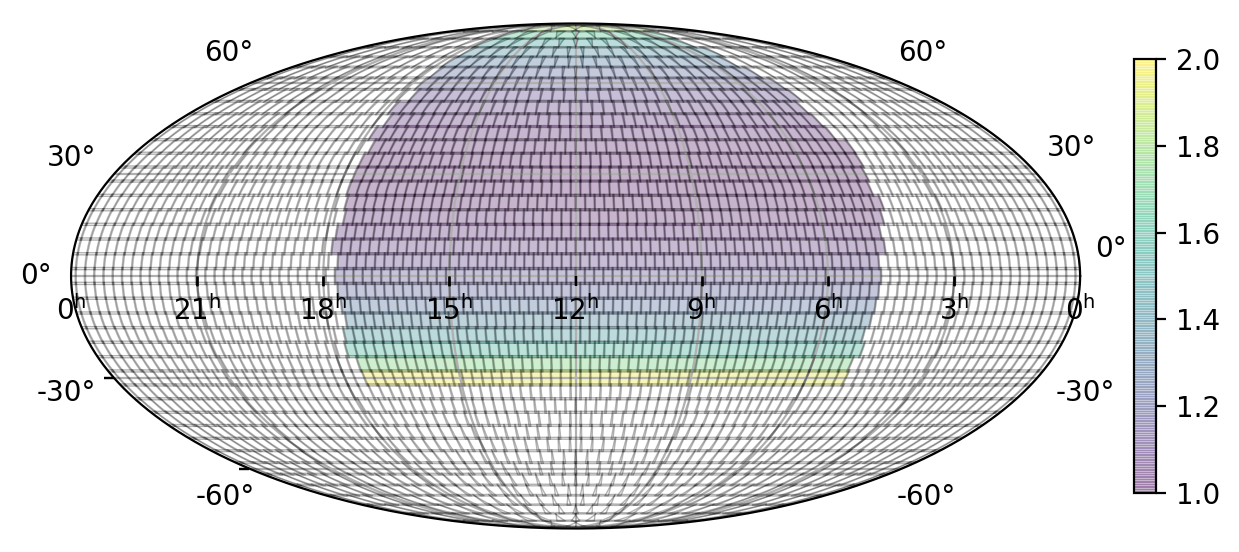
\includegraphics[width=0.7\linewidth]{images/survey_sims/30_1N4_meridian_airmass.png}
    \end{center}

    \caption[Mean observation airmasses using the meridian scanning method]{
        Mean observation airmasses for the first month of a survey using the meridian scanning method, restricting observations to tiles within $\pm\SI{10}{\degree}$ of the meridian. With the limit the airmass of observations can be optimised, but the coverage of the survey is reduced.
    }\label{fig:survey_sim_airmass_meridian}
\end{figure}

\clearpage

\begin{table}[t]
    \begin{center}
    \begin{tabular}{c|cc|c|c|c} % chktex 44

    Survey &
    \multicolumn{2}{c|}{Fraction of sky observed} &
    Mean cadence &
    Mean observed
    \\
    method &
    1st month &
    whole year &
    (days) &
    airmass
    \\
    \midrule
    Meridian  \SI{\pm5}{\degree} & 39.4\% & 76.5\% &  $6.2\pm0.5$ & $1.2\pm0.2$ \\
    Meridian \SI{\pm10}{\degree} & 41.3\% & 76.5\% &  $6.6\pm0.7$ & $1.2\pm0.3$ \\
    Meridian \SI{\pm30}{\degree} & 48.5\% & 76.5\% &  $7.9\pm0.8$ & $1.3\pm0.3$ \\
    Meridian \SI{\pm45}{\degree} & 53.3\% & 76.5\% &  $8.8\pm0.9$ & $1.3\pm0.3$ \\
    No limit                     & 57.0\% & 76.5\% & $10.1\pm1.8$ & $1.6\pm0.3$ \\

    \end{tabular}
    \end{center}
    \caption[Comparison of survey simulations using a meridian limit]{
        Comparison of 1N4 survey simulations using different meridian limits.
    }\label{tab:survey_sim_meridian}
\end{table}

As intended by restricting observations to be closer to the meridian the mean airmass of the observations is decreased. This is shown by the mean airmasses in \aref{tab:survey_sim_meridian} but is even clearer in the distributions shown in \aref{fig:survey_sim_airmass_365}. The optimal value of the meridian limit will depend on several factors, including what the number of telescopes being used (as the instantaneous field of view increases the tiles within the strip will be observed faster, and so the meridian limit should be increased).

A side effect of this method is that as the width of the meridian strip is decreased and the effective visible sky is reduced each tile within the strip is observed more often, and therefore the mean cadence decreases. However it also leads to fewer unique tiles being observed, as shown by the fraction of sky observed within a single month reducing from near to 60\% using the previous method to almost to 40\% with a strict limit. This has a knock-on effect on the effectiveness of the project, as while optimal data quality is a good intention recent observations of tiles are still required for the difference imaging process. In practice it might be necessary to have two concurrent surveys, one optimised for quality by being limited to the meridian strip and the other optimised for coverage with no such limit.

Overall while more work is required these simulations are a good test to show that more advanced scheduling strategies could be developed in the future, in order to further optimise the \gls{gtecs} scheduling system for the all-sky survey.

\end{colsection}

% ~~~~~~~~~~~~~~~~~~~~

\end{colsection}

% ########################################
